\documentclass[11pt]{article}

% =========================================================
% ENCODING AND TYPOGRAPHY
% =========================================================
\usepackage[T1]{fontenc}
\usepackage[utf8]{inputenc}
\usepackage{lmodern}
\usepackage{microtype}

% =========================================================
% PAGE LAYOUT
% =========================================================
\usepackage[
    a4paper,
    top=2.6cm,
    bottom=2.6cm,
    left=2.8cm,
    right=2.8cm
]{geometry}

\usepackage{setspace}
\setstretch{1.05}

\setlength{\parindent}{0pt}
\setlength{\parskip}{0.55em}

% =========================================================
% MATHEMATICS
% =========================================================
\usepackage{amsmath}
\usepackage{amssymb}
\usepackage{mathtools}

% =========================================================
% TABLES
% =========================================================
\usepackage{booktabs}
\usepackage{array}
\usepackage{tabularx}

\renewcommand{\arraystretch}{1.12}

% =========================================================
% FIGURES
% =========================================================
\usepackage{graphicx}
\usepackage{float}

\graphicspath{
    {newsections/images/}
}

% =========================================================
% CAPTIONS
% =========================================================
\usepackage[
    font=small,
    labelfont=bf,
    justification=justified,
    singlelinecheck=false
]{caption}

% =========================================================
% LISTS
% =========================================================
\usepackage{enumitem}

\setlist[itemize]{
    leftmargin=1.5em,
    itemsep=0.3em,
    topsep=0.4em
}

\setlist[enumerate]{
    leftmargin=1.7em,
    itemsep=0.3em,
    topsep=0.4em
}

% =========================================================
% SECTION FORMATTING
% =========================================================
\usepackage{titlesec}

\titleformat{\section}
    {\large\bfseries}
    {\thesection}
    {0.8em}
    {}

\titleformat{\subsection}
    {\normalsize\bfseries}
    {\thesubsection}
    {0.8em}
    {}

\titleformat{\subsubsection}
    {\normalsize\itshape}
    {\thesubsubsection}
    {0.8em}
    {}

\titlespacing*{\section}
    {0pt}{2.2em}{0.8em}

\titlespacing*{\subsection}
    {0pt}{1.7em}{0.6em}

\titlespacing*{\subsubsection}
    {0pt}{1.3em}{0.5em}

% =========================================================
% CITATIONS AND REFERENCES
% =========================================================
\usepackage[
    authoryear,
    square
]{natbib}

% =========================================================
% COLOURS AND LINKS
% =========================================================
\usepackage{xcolor}

\definecolor{linkblue}{RGB}{35,70,110}
\definecolor{citeblue}{RGB}{45,80,120}

% Editorial change marks (for the review copy only).
% In the final clean copy, change the definition to: \newcommand{\rev}[1]{#1}
\definecolor{revisionblue}{RGB}{15,81,164}
\newcommand{\rev}[1]{{\color{revisionblue}#1}}

\usepackage[
    colorlinks=true,
    linkcolor=linkblue,
    citecolor=citeblue,
    urlcolor=linkblue,
    pdfborder={0 0 0}
]{hyperref}

% =========================================================
% HEADER AND FOOTER
% =========================================================
\usepackage{fancyhdr}

\pagestyle{fancy}
\fancyhf{}

\fancyhead[L]{\small Text-based Entity Resolution}
\fancyhead[R]{\small Ahmed et al.}

\fancyfoot[C]{\thepage}

\renewcommand{\headrulewidth}{0.4pt}
\renewcommand{\footrulewidth}{0pt}

\setlength{\headheight}{14pt}

% No header on the title page
\fancypagestyle{plain}{
    \fancyhf{}
    \fancyfoot[C]{\thepage}
    \renewcommand{\headrulewidth}{0pt}
}

% =========================================================
% DOCUMENT
% =========================================================
\begin{document}

% ---------------------------------------------------------
% TITLE
% ---------------------------------------------------------

\title{
    \vspace{-1.2cm}
    \textbf{\LARGE Text-based Entity Resolution Using Transformer Models}
}

\author{
    Abrar Ahmed MSc
    \and
    Professor Li-Chun Zhang
    \and
    Prof. Dr. Ralf Münnich
    \and
    Prof. Dr. Martin Vogt
}

\date{July 21, 2026}

\maketitle

\vspace{-0.5em}

% ---------------------------------------------------------
% ABSTRACT
% Keep unchanged for now.
% We will revise the abstract after the main paper is final.
% ---------------------------------------------------------

\begin{abstract}

Entity resolution (also known as record linkage) aims to classify which database
items, or file records, refer to the same entity, where the entity is typically a
real-world object such as a person, business or product. Transformer models have
brought artificial intelligence to text-based entity resolution through their
superior ability for natural language processing. However, applying a transformer
model directly to ``link or not to link'' a large number of record pairs can be
computationally too costly in practice. We propose a workflow of text-based entity
resolution that extends traditional approaches to record linkage by incorporating
judicious uses of transformer models. A bi-encoder is used for text embedding and
blocking, while traditional generative or discriminative models can be used for
scoring and classification. A cross-encoder can then be reserved for selected harder
cases, providing a mechanism for trading linkage accuracy against computational cost.
We also discuss fine-tuning and provide a workable approach to linkage error
assessment for the combined procedure. The proposed workflow is evidenced and
illustrated using two benchmark datasets from the Magellan data repository.

\end{abstract}

% ---------------------------------------------------------
% CONTENTS
% ---------------------------------------------------------

\tableofcontents
\clearpage

% =========================================================
% SECTION 1
% Introduction
%
% Keep Zhang's content essentially unchanged.
% =========================================================

% ============================================================
%  Section — Introduction
% ============================================================

\section{Introduction}
\label{sec:introduction}

The task of entity resolution is to classify the database items (or file records) that refer to the same entity \citep{christen2012data}, where the entity may be person, business, product, etc. In this context, any two items corresponding to the same entity are said to form a \emph{match}, whereas the two items may or may not be classified as a \emph{link} at the result of entity resolution. The need of entity resolution arises in official statistics, machine learning, research or knowledge synthesis, and many other areas, where it is often the prerequisite of downstream tasks that treat the linked dataset as a single source of input. 

Record linkage across two files is a typical problem of entity resolution \citep[e.g.][]{fellegi1969theory, newcombe1959automatic, jaro1989advances, lee2021maximum}. Instead of hand-crafted rules for link classification, the probabilistic approach asks one to model the distortions of the linkage key variables, or simply \emph{keys}, such as (name, date-of-birth, address) for records of persons, so that the decision whether or not to link two records can be largely or entirely data-driven (i.e. without the need for clerical review).

\begin{figure}[ht]
\centering
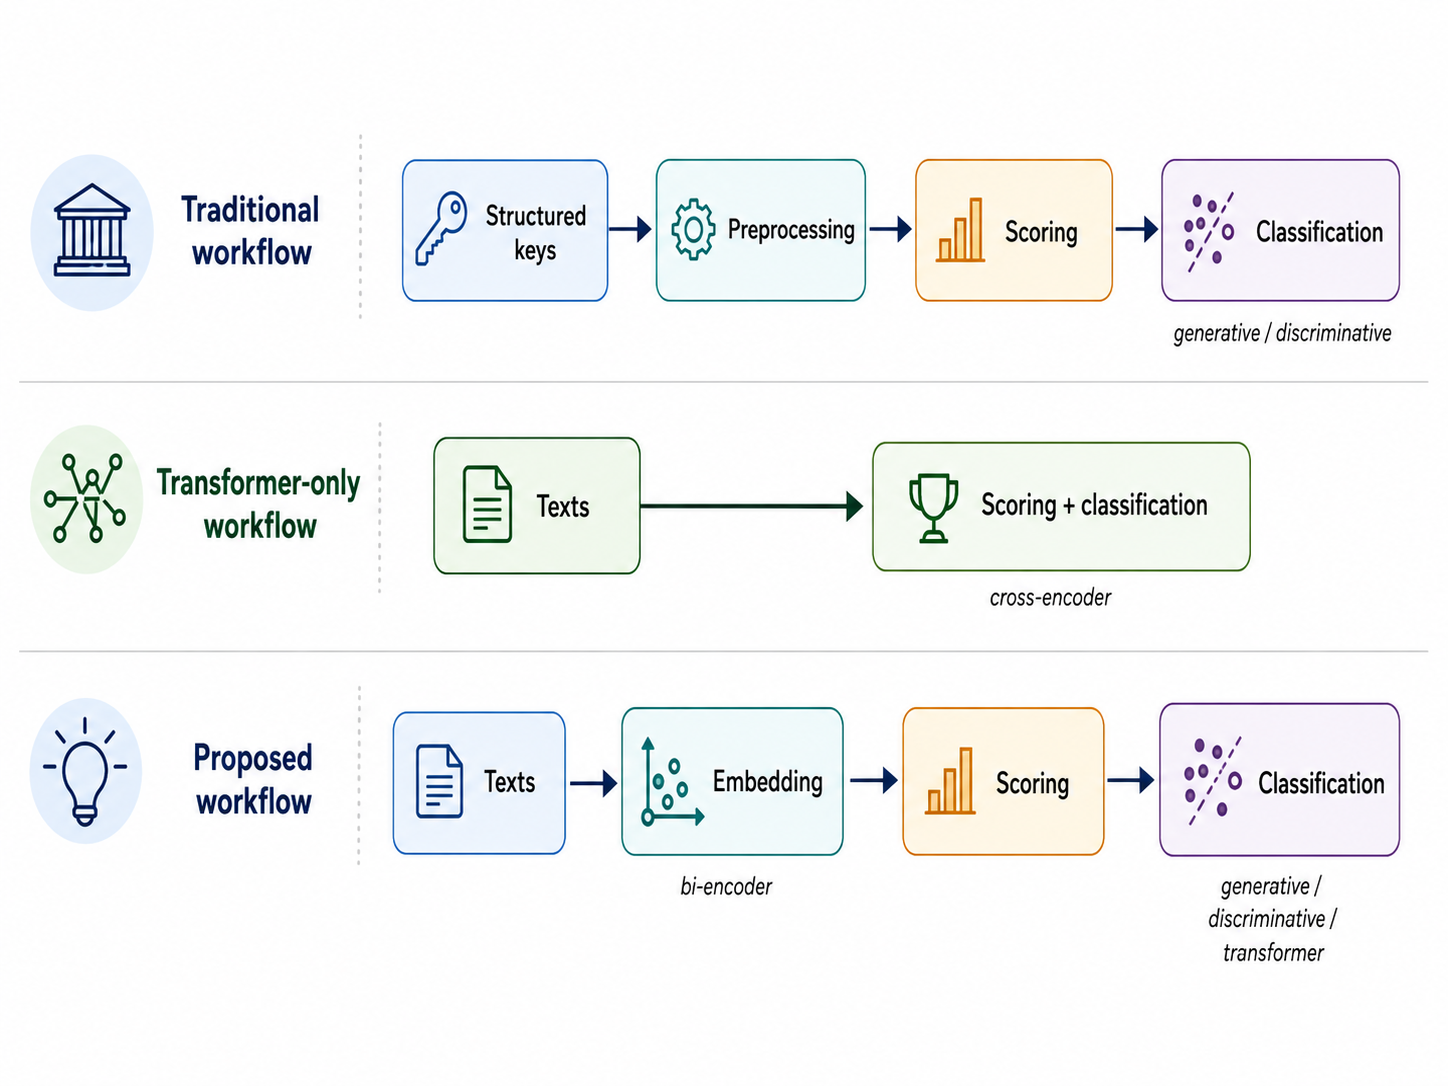
\includegraphics[width=0.85\textwidth]{newsections/images/image_1.png}
\caption{Workflows of entity resolution. Traditional workflow (top), transformer-only workflow (middle), and proposed workflow (bottom).}
\label{fig:workflow}
\end{figure}

The traditional workflow of probabilistic linkage may be given generically as in Figure \ref{fig:workflow}. Although the key values are given as structured data, preprocessing is often necessary to accommodate typical variations of the same key, such as different spellings of an address or name. Scoring then refers to the statistical modelling of the key-value distortions. Two possibilities may be considered.

\begin{itemize}[leftmargin=6mm,itemsep=0pt]

\item Generative models have been common ever since \citet{fellegi1969theory}, where one models the probability of the observed key-value agreement pattern of a pair of records given that they form a match, and the probability given that they do not form a match. The ratio of these two probabilities forms the basis for link classification.

\item Discriminative models target the probability that a pair of records form a match given their observed key values or key-value agreement pattern. While uncommon for record linkage in the unsupervised setting, these models arise naturally in the supervised setting where labelled matches are available. Logistic regression, which we consider later in this paper, is one such model.

\end{itemize}

Finally, \citet{fellegi1969theory} use the likelihood ratio resulting from generative models to classify links and non-links directly, leaving a subset of record pairs to be decided by clerical review. \citet{lee2021maximum} propose maximum entropy classification (MEC) for record linkage based on generative models, which enables fully automated link classification guided by the estimated rates of false links and missing matches.

\begin{table}[ht]
\centering
\caption{Examples of item descriptions in the DBLP-Scholar and Abt-Buy datasets.}
\begin{tabular}{l | l}
\toprule
Field & DBLP-Scholar text \\
\midrule
Title & Distributed Representations of Tuples for Entity Resolution \\
Author & Z Ebraheem, Thirumuruganathan, S. Joty \\
Venue & Proc. VLDB Endow. \\
Year & 2018 \\
\midrule
Field & Abt-Buy text \\
\midrule
Name & Sony Black Pocket AM/FM Walkman Radio - SRF59 \\
Description & Belt Clip Included / Uses 1 AA Battery / Local/DX Switch... \\
\bottomrule
\end{tabular}
\label{tab:text}
\end{table}

However, for entity resolution based on messy texts instead of structured key values, it is often difficult and ineffective to formulate deterministic rules of preprocessing. Table \ref{tab:text} gives two examples, one from the DBLP-Scholar dataset and the other from the Abt-Buy dataset, both in the Magellan data repository of benchmark datasets for entity resolution \citep{konda2016magellan}; see Appendix \ref{app:datasets} for details.

The text data in DBLP-Scholar are structured in four fields. Although the content can be quite noisy for some fields, such as author names, one might still attempt preprocessing of these texts by hand-crafted rules. In contrast, the relatively free-form texts in the Abt-Buy dataset may be highly irregular from one product to another, and it is not obvious that traditional preprocessing rules for keys such as name and address would be effective for the product names and descriptions here.

It is therefore natural to consider machine learning models that can work directly with such text. \citet{mudgal2018deep} show that deep-learning models can outperform hand-crafted feature engineering for text-based entity resolution. More recently, transformer models, introduced by \citet{vaswani2017attention}, have provided a way to represent and compare texts while taking their context into account. The transformer architecture uses self-attention to model relationships between tokens within a sequence, which makes it particularly suitable for handling textual data.

In the work of \citet{li2020deep}, entity resolution is cast as a sequence-pair classification task using a pretrained transformer language model. The two records are supplied jointly to the model, allowing the self-attention layers to represent interactions across the paired input. This type of architecture is commonly referred to as a \emph{cross-encoder}.

The computational cost becomes prohibitive, however, if the cross-encoder is applied to every possible pair of records, as we shall illustrate later using the DBLP-Scholar and Abt-Buy datasets. A \emph{bi-encoder} transformer model \citep{reimers2019sentence, wang2022sudowoodo} instead encodes each text separately as a numerical vector, or \emph{embedding}. Similarity between these embeddings can then be used to identify a much smaller set of candidate records before more expensive scoring or classification is applied. This provides a form of semantic blocking, analogous to traditional blocking in record linkage. For instance, \citet{reimers2019sentence} report that finding the most similar pair in a collection of $10{,}000$ sentences required about 65 hours with a standard BERT model, compared with about 5 seconds using SBERT embeddings and cosine similarity.

Bi-encoder blocking greatly reduces the number of record pairs that require further comparison, but it still leaves several choices about how the candidate pairs should be scored and classified. In particular, the numerical representations produced by a bi-encoder can be combined with traditional generative or discriminative scoring methods, or the candidate texts can be passed to a cross-encoder for classification. The usefulness of these alternatives may also change after the transformer models are fine-tuned to the texts of a particular application. These considerations motivate the integrated workflow in Figure \ref{fig:workflow}, as well as a closer examination of the linkage errors associated with the resulting models.


\subsection{Proposed workflow using transformer models}
\label{sec:proposal}

Our proposed workflow for entity resolution is given in Figure \ref{fig:workflow}, which uses transformer models as well as traditional generative or discriminative models.

While the workflow is applicable to both the supervised and unsupervised settings, i.e. with or without a sample of labelled matches, we shall focus on the supervised setting in this paper. Transformer models are considered for embedding and classification. Notice that cross-encoder models with text as input are not relevant for scoring given numerical embeddings, whereas how to use transformer models to achieve scoring-classification from texts directly remains an open question in the unsupervised setting.

A fundamental difficulty for modelling arises from the following fact about entity resolution. While matched items refer to real entities, a pair of non-matches does not correspond to a single real entity. For instance, when two records refer to two different persons, there is no person associated with both records. It follows that there is no naturally defined population of non-matches corresponding to the population of matches, which complicates the construction of training data for supervised learning.

To deal with this difficulty, it is common to create the training and test sets in a way that
mirrors how the models will later be applied to out-of-sample items. Suppose that, for each
out-of-sample record in $A$, one would conduct blocking to gather $k$ candidate records in
$B$ for scoring and classification. We then construct candidate records in the same manner
for the sampled file-$A$ records, and partition those file-$A$ records into training and test
sets together with their associated candidate records. Thus, all candidate pairs associated
with a given file-$A$ record remain in the same partition. Duplication of candidate records
for different records in $A$ is allowed if it is also allowed for the out-of-sample records in
application.

Notice that, if none of the valid matched records is selected among the $k$
candidates, the corresponding file-$A$ record cannot be linked correctly. Hence the
choice of $k$ induces a floor of missing match rate (MMR). In practice, for scoring
and classification, it is natural to select the $k$ most likely link candidates for
blocking, i.e. the records in $B$ with the most similar texts, and to choose $k$ such
that the MMR floor is considered acceptable. Selecting the most similar candidates
also provides more difficult non-matches for supervised learning than selecting
non-matches randomly.

In addition to the MMR, another central performance measure is the \emph{false linkage rate (FLR)}. We use the FLR and MMR, following the definitions of \citet{lee2021maximum}, for the evaluation and comparison of the different methods considered in this paper. Their formal definitions in the present setup are given in Section \ref{sec:setting}. Notice that both are well-defined whether or not one employs additional treatments of duplicated candidate records for scoring and classification.

The details of the steps in the proposed workflow will be studied in this paper, and the relevant methodological choices exemplified and compared.


 

\subsection{Link classification errors by transformer models}
\label{sec:literature:error}

The estimation of FLR and MMR for link classification based on transformer models requires special attention.

\rev{If one uses only a pretrained transformer model that is fixed independently of the labelled data, then, under the SRSWOR assumption stated in Section~\ref{sec:setting}, the observed errors in the labelled file-$A$ sample may be used to estimate the FLR and MMR that would arise over the corresponding finite population of file-$A$ records. This population interpretation is conditional on the labelled records being a probability sample from that population. In the benchmark experiments below, by contrast, the available benchmark data are partitioned internally into training and test sets. The resulting FLR and MMR are therefore internal test-set quantities; they should not be interpreted directly as design-based estimates for a wider operational database unless the stated sampling assumption holds.}

The matter becomes more complicated when the transformer model is fine-tuned using the labelled sample. An obvious approach is to split the labelled sample into a training set for fine-tuning and a test set for estimating the errors of the resulting subsample-tuned model. This is valid if one is willing to apply that subsample-tuned model directly to the out-of-sample items. It is not sufficient, however, if the subsample training is used only to determine the hyperparameters of fine-tuning, after which the transformer model is fine-tuned again using the entire labelled sample and this final model is applied to the remaining records. The errors observed on the original test set then refer to a different fitted model from the one eventually used for entity resolution.

We shall study this issue later using the DBLP-Scholar and Abt-Buy datasets, illustrating both the statistical problem and the practical difficulties that arise. Below we briefly explain why the issue also presents difficulties for several existing approaches to error assessment.

\emph{Bayesian uncertainty propagation.}
In Bayesian approaches to entity resolution, one may model the key values or their disagreement patterns and generate link sets according to the posterior distribution of the matches, conditional on the observed keys; see, for example, \citet{tancredi2011hierarchical, sadinle2017bayesian, steorts2016bayesian}. It is unclear how such prior-posterior uncertainty propagation can be carried through a fine-tuned transformer model, which does not provide the likelihood function required for the corresponding Bayesian calculation. Moreover, repeatedly generating link sets while refitting or evaluating a large transformer model would be computationally expensive.

\emph{Auditing.}
A practical approach in the unsupervised setting of entity resolution is to draw an audit sample from the classified links in order to estimate the FLR \citep{christen2012data}; see also \citet{binette2024evaluation} for a more elaborate proposal. In the supervised setting, the labelled match sample can be used to estimate both FLR and MMR when the classification model is fixed independently of that sample. The situation changes when the same labelled observations are used for fine-tuning. Auditing additional out-of-sample records could provide information about the final model, but identifying their true matches may require substantial clerical effort.

\emph{Design-based sample inference.}
\citet{zhang2025predictive, zhang2026debiasing} develop unbiased estimation of algorithmic prediction or classification errors under finite population sampling. In principle, this provides a way to accommodate models trained using sampled observations. In practice, however, the required calculations can be costly for transformer models. Moreover, although link classification can be viewed as a special case of classification, unbiased estimation of classification errors in this framework relies on randomised prediction or classification, whereas deterministic classification is generally preferred for record linkage.




\subsection{Notations and rest of paper}
\label{sec:setting}

Let us now introduce the basic notations related to the workflow of entity resolution, formalising the concepts discussed above and preparing for the investigations later.

Without loss of generality, let us use the standard setup of record linkage across two files. Let
$A = \{a_1, \ldots, a_{n_A}\}$ and
$B = \{b_1, \ldots, b_{n_B}\}$
be two files containing $n_A$ and $n_B$ records, respectively. Let entity resolution, or record linkage, be based on
$\{\tau_i : i \in A \cup B\}$,
where $\tau_i$ is the text associated with record $i$, which may or may not consist of structured fields, as exemplified in Table \ref{tab:text}.

Let $M$ be the set of matches, $M \subset A \times B$, and denote a match by $(i,j) \in M$, or equivalently $y_{ij}=1$, if records $i$ and $j$ refer to the same entity. A non-match is denoted by $(i,j) \notin M$, or $y_{ij}=0$. Let $A(M)$ and $B(M)$ denote the records in $A$ and $B$, respectively, belonging to $M$.

Let $A_s\subseteq A$ denote the sampled file-$A$ records. For simplicity of
exposition in this paper, we assume that $A_s$ is obtained from $A$ by simple random
sampling without replacement (SRSWOR). Let

\[
s_M=\{(i,j)\in M:i\in A_s\}
\]

denote the labelled match relation induced by these sampled records. Let $A(s_M)$
denote the records in $A_s$ having at least one match in $s_M$, and let $B(s_M)$
denote the corresponding matched records in $B$. Thus,
$A_s\setminus A(s_M)$ contains the sampled file-$A$ records that are non-matchable.

In practice, one first draws the file-$A$ records in $A_s$ and then identifies all
their known matches by any means necessary. This formulation samples file-$A$
records rather than individual matched pairs. The distinction becomes relevant when
a file-$A$ record has more than one valid partner in $B$.

To limit the number of comparisons for the models, let $C_i$ denote the block of candidate records for each $i \in A$ according to a given blocking scheme, where
$C_i \subset B$, and $C_i \cap C_j$ may be non-empty for $i \neq j \in A$. Let $k$ be the size of $C_i$ in the case $|C_i| \equiv k$.

By applying a \emph{given} model of link classification to
\[
\{(i,j) : i \in A_s,\; j \in C_i\},
\]
denote by $\ell_i=1$ if $i \in A_s$ is linked and $\ell_i=0$ if it is not linked. One can estimate the FLR and MMR when the model is applied to all the record pairs
\[
\{(i,j) : i \in A,\; j \in C_i\},
\]
as
\begin{equation}
\label{eq:FLR:MMR}
\widehat{\mathrm{FLR}}
=
1-
\frac{
\sum_{i \in A(s_M)} \ell_i y_{ij_i}
}{
\sum_{i \in A_s} \ell_i
},
\qquad
\widehat{\mathrm{MMR}}
=
1-
\frac{
\sum_{i \in A(s_M)} \ell_i y_{ij_i}
}{
|A(s_M)|
},
\end{equation}
where $j_i$ refers to the linked record in $B$ given $\ell_i=1$, and
$y_{ij_i} \equiv 0$ if $i \in A \setminus A(M)$.

For supervised learning including non-matches in addition to matches, let
$(A_1,A_2)$ denote a partition of $A_s$, where

\[
A_1\cup A_2=A_s,
\qquad
A_1\cap A_2=\emptyset.
\]

We use $A_1$ for training and $A_2$ for testing. Let

\[
s_r=\{(i,j)\in s_M:i\in A_r\},
\qquad r=1,2,
\]

denote the labelled match relations induced by these two sets of file-$A$ records.
Thus, all known matches belonging to the same file-$A$ record remain on the same
side of the training-test partition.

According to the setup in Section 1.1, the corresponding candidate non-matches
associated with matchable records are

\[
\bigcup_{i\in A_1\cap A(s_M)}
\{(i,j):j\in C_i,\ y_{ij}=0\}
\]

for training and

\[
\bigcup_{i\in A_2\cap A(s_M)}
\{(i,j):j\in C_i,\ y_{ij}=0\}
\]

for testing. For non-matchable sampled file-$A$ records, all candidate pairs are
non-matches, giving

\[
\bigcup_{i\in A_r\setminus A(s_M)}
\{(i,j):j\in C_i\},
\qquad r=1,2.
\]

Notice that the setup of supervised learning above can vary with the blocking scheme. In particular, given the fixed block size $k$, we consider two schemes.

\begin{itemize}[leftmargin=2mm,itemsep=0pt]

\item[] \emph{Scheme-I}: for each $i \in A(s_M)$, let $C_i$ contain one retained matched record $j$ for which $(i,j) \in s_M$, together with $k-1$ non-matches.

\item[] \emph{Scheme-II}: for each $i \in A(s_M)$, let $C_i$ consist of the $k$ most similar file-$B$ records.

\end{itemize}

Under Scheme-I, the retained labelled match is inserted into each candidate block, whereas under
Scheme-II the candidate block is determined entirely by similarity and may therefore fail
to contain a valid match. The difference between the two schemes decreases as the block
size $k$ increases. Scheme-I makes more efficient use of the labelled matches for learning,
while Scheme-II is more closely related to the application of the models to out-of-sample
records.

In the experiments below we use Scheme-II to construct the candidate blocks. For supervised
fitting, however, one known valid file-$B$ partner is retained as the positive example for each
matchable file-$A$ record, whether or not that particular retained partner occurs in $C_i$.
The non-match examples are drawn from $C_i$, with every known valid partner excluded from
the non-match class. At evaluation, $C_i$ is not augmented in this way: a predicted link must
be selected from the retrieved candidate block, and failure to retrieve any valid partner
contributes to the floor MMR.

Section \ref{sec:experimental-setup} describes the datasets and experimental setup used throughout the empirical analysis. We study the proposed workflow using pretrained transformer models in Section \ref{sec:pretrained}. Section \ref{sec:finetuning} considers the fine-tuning of transformer models, including the related assessment of link classification errors. Section \ref{sec:final-remarks} provides the final remarks and discusses topics for future research and development.




% =========================================================
% SECTION 2
% Workflow with pretrained transformer models
%
% Active revision begins here.
% =========================================================

\section{Data and experimental setup}
\label{sec:experimental-setup}

\subsection{Datasets and preprocessing}
\label{sec:data}

We use the DBLP-Scholar and Abt-Buy datasets from the Magellan repository
\citep{konda2016magellan}. The two datasets differ considerably in both scale and
the form of their textual information. DBLP-Scholar contains bibliographic records,
whereas Abt-Buy contains product records collected from two online retailers.
\rev{Our evaluation reformulates these benchmark datasets as record-level candidate
retrieval and linkage problems, with FLR and MMR calculated over file-$A$ records and
their candidate sets. These error rates are therefore not directly comparable to the
pair-level precision, recall or F1 scores reported under the standard entity-matching
classification protocol in, for example, DeepMatcher and Ditto
\citep{mudgal2018deep,li2020deep}.}
Table \ref{tab:dataset-summary} summarises the data used in the experiments.

\begin{table}[ht]
\centering
\caption{Summary of the datasets used in the experiments.}
\begin{tabular}{lrrrr}
\toprule
Dataset & $n_A$ & $n_B$ & Gold pairs & Matchable records in $A$ \\
\midrule
DBLP-Scholar & 2,616 & 64,263 & 5,347 & 2,408 \\
Abt-Buy      & 1,081 & 1,092  & 1,097 & 1,081 \\
\bottomrule
\end{tabular}
\label{tab:dataset-summary}
\end{table}

For DBLP-Scholar, file $A$ is the DBLP file and file $B$ is the Scholar
file. The original files contain the fields title, authors, venue and year.
The gold-standard mapping contains 5,347 pairs involving 2,408 distinct
DBLP records and 5,218 distinct Scholar records. A DBLP record may therefore
have more than one valid Scholar partner. Of the 2,616 DBLP records, 2,408
have at least one gold-standard match.

For Abt-Buy, file $A$ is the Abt file and file $B$ is the Buy file. The
original Abt file contains the product name, description and price, while the
Buy file additionally contains the manufacturer. The gold-standard mapping
contains 1,097 pairs. All 1,081 Abt records have at least one known match in
the Buy file, and some records have more than one valid partner.

For semantic blocking, we use the title field for DBLP-Scholar and the
product-name field for Abt-Buy. These fields contain no missing values in
either dataset. The other common text fields remain available for the field-level comparisons
used by the traditional scoring models. The complete
gold-standard mappings are retained when determining whether a candidate
set contains a valid match and when evaluating a predicted link.

For constructing supervised match examples, one valid file-$B$ partner is
retained for each matchable file-$A$ record. Thus, there are 2,408 retained
positive pairs for DBLP-Scholar and 1,081 for Abt-Buy. Importantly, the
other known valid partners are not treated as non-matches. At evaluation,
a predicted link is considered correct if the selected file-$B$ record is
any known valid partner of the corresponding file-$A$ record.


\subsection{Training and candidate construction}
\label{sec:training-candidates}

The experimental unit is a file-$A$ record together with its candidate
file-$B$ records, rather than an individual candidate pair. This distinction
is important because all the pairs associated with a given file-$A$ record
must remain together when the data are divided into training and test sets.

For the main experiments, the file-$A$ records are randomly divided 50--50
into training and test sets. In DBLP-Scholar this gives 1,308 records in
each half. In Abt-Buy, 540 records are assigned to training and 541 to
testing. The primary results reported in Sections 3 and 4 use random seeds
42, 43 and 44 and are averaged over the three resulting splits. \rev{In Tables
\ref{tab:comparison}--\ref{tab:discrimination-gap}, numbers in parentheses are
Monte Carlo standard errors, calculated as the sample standard deviation of
the three seed-level error rates divided by $\sqrt{3}$. The FLR and MMR
are calculated separately for each split before averaging. With only three
replications, these standard errors describe observed split-to-split
variation and do not support precise interpretation of small method differences.}
Seeds 45--51 are used later where additional Monte Carlo replications are
required.

Candidate blocks are constructed according to Scheme-II in Section 1.3.
First, the pretrained bi-encoder \texttt{all-MiniLM-L6-v2} is used to
embed the blocking text of every record in files $A$ and $B$. For each
record $i\in A$, the records in $B$ are ranked by cosine similarity of
their embeddings, and the $k$ most similar records form $C_i$. We consider
primarily $k=5$ and $k=50$, while $k=1$ is also useful for examining the
blocking floor.

The same procedure is applied independently to every file-$A$ record.
Consequently, the same file-$B$ record may occur in the candidate blocks
of several file-$A$ records. This mirrors how semantic blocking would be
applied to records outside the labelled sample and avoids imposing an
artificial one-to-one restriction at the blocking stage.

The labelled candidate pairs are then constructed for supervised learning. Each retained
valid partner provides one positive example for its matchable file-$A$ record. This retained
positive is supplied for supervised fitting whether or not that particular partner occurs
among the retrieved top-$k$ candidates. The non-match examples are drawn from the
retrieved candidate block: candidate-derived pairs that are not known valid partners are
treated as negatives, while every additional gold-standard partner of the same file-$A$
record is excluded from the non-match class. Thus, one retained positive may be accompanied
by several retrieved hard non-matches rather than by only one negative example. At
evaluation, the candidate block is not augmented with the retained positive, so a record
cannot be linked correctly when none of its valid partners has been retrieved. The resulting
non-matches are therefore relatively difficult examples selected by semantic similarity
rather than arbitrary pairs drawn from $A\times B$.

For DBLP-Scholar, the training and test sets also contain file-$A$ records
that have no gold-standard partner. Their candidate pairs are all
non-matches. This is useful because such records occur in the application
of record linkage and a classification procedure should be able to leave
them unlinked. For Abt-Buy, every file-$A$ record has at least one known
valid partner.

For discriminative link classification, the candidate pairs belonging to
the training half are further divided 80--20 into fitting and validation
parts. The fitting part is used to estimate the model and the validation
part to choose the link-classification threshold by maximising the F1
score. The outer test records are not involved in this choice.


\subsection{Models and implementation}
\label{sec:models-implementation}

We consider three ways of progressing from the candidate pairs to link
classification, corresponding to the workflows introduced in Figure
\ref{fig:workflow}.

In the traditional workflow, field-level text comparisons are obtained
with the Jaro--Winkler metric. In the proposed workflow, these are replaced
by cosine similarities calculated from bi-encoder embeddings. Unless
otherwise stated, the bi-encoder is
\texttt{all-MiniLM-L6-v2} \citep{reimers2019sentence}. Section
\ref{sec:embedding-scoring} explains how these comparison outcomes enter
the subsequent scoring models.

Two traditional scoring models are used in the main comparison. The
generative model follows the MEC approach of \citet{lee2021maximum},
with the match and non-match densities of the continuous comparison
outcomes estimated by kernel density estimation. The discriminative model
is logistic regression. A radial-kernel SVM, XGBoost and a small
multilayer perceptron are considered later as a sensitivity analysis.

For direct classification from paired texts, we use the cross-encoder
\texttt{ms-marco-MiniLM-L-6-v2}. Both transformer models are first
considered in their pretrained form. Their fine-tuning is then investigated
in Section \ref{sec:fine-tuning-models}, where we give the corresponding
training settings and explain how the candidate blocks are treated before
and after fine-tuning.

For discriminative models, including the cross-encoder, a validation
subset of the training pairs is used to choose the threshold for declaring
a link by maximising the F1 score. The particular classification rules are
described together with the corresponding models below, since they form
part of the methodological comparison rather than merely an implementation
detail.

The objective of these experiments is not to identify the best possible
model or hyperparameter configuration for either benchmark dataset.
Rather, the common setup enables us to examine how embedding, scoring,
classification and fine-tuning can be combined within the proposed
workflow. \rev{Accordingly, the reported error rates are intended to illustrate the
behaviour of this workflow under a common experimental setup, rather than to
establish state-of-the-art entity-matching performance or a benchmark ranking
against published systems such as DeepMatcher \citep{mudgal2018deep}, Ditto
\citep{li2020deep}, or the method of \citet{peeters2021dual}.}


\subsection{Evaluation}
\label{sec:evaluation}

The unit of link classification is again a file-$A$ record. Given the
candidate block $C_i$, a scoring model ranks or scores its candidate
file-$B$ records. If a link is declared, let $j_i$ denote the selected
record. For models that use a classification threshold, no link is
declared when the best candidate does not satisfy that threshold. The
generative MEC calculations considered below instead select the
highest-ranked candidate according to the estimated density ratio.

A declared link is counted as correct whenever $(i,j_i)$ is one of the
known gold-standard pairs for record $i$. This is important for both
datasets because the gold-standard relation need not be one-to-one.
Selecting a valid partner other than the particular partner retained for
supervised fitting is therefore still a correct link.

The two error measures are the FLR and MMR defined in Equation (1).
It is useful to state their empirical calculation explicitly. Let $D$
be the number of links declared among the test file-$A$ records, let
$C$ be the number of those declarations that select a valid
gold-standard partner, and let $M$ be the number of matchable file-$A$
records in the test set. Then

\[
\widehat{\mathrm{FLR}}
=
1-\frac{C}{D},
\qquad
\widehat{\mathrm{MMR}}
=
1-\frac{C}{M}.
\]

Thus, an incorrect declared link contributes to both error measures:
it is a false link among the declarations and, for a matchable
file-$A$ record, it also means that the true match has not been
recovered. An undeclared matchable record contributes to the MMR but
not to the numerator or denominator of the FLR. For DBLP-Scholar,
a declared link for a non-matchable file-$A$ record is necessarily a
false link and therefore contributes to the FLR.

Blocking imposes an additional lower bound on the MMR. If none of the
valid partners of a matchable file-$A$ record occurs in $C_i$, no
scoring or classification model operating on that block can link the
record correctly. We refer to the proportion of such records as the
floor MMR and examine it explicitly in Section
\ref{sec:embedding-scoring}.

Unless otherwise stated, the tables in Sections 3 and 4 report the mean
FLR and MMR over the three primary random splits. In the later
investigation of training-set fractions and subsample error assessment,
seeds 42--51 provide ten Monte Carlo replications. There we additionally
report Monte Carlo standard errors, and, where relevant, relative Monte
Carlo standard errors, in order to distinguish variation across random
splits from the differences between modelling procedures.

\rev{The replication counts were not selected to attain a prespecified
hypothesis-testing power or precision target. They reflect the computational
cost of repeated fine-tuning and the descriptive purpose of the experiments.
Accordingly, the three-split comparisons in Tables
\ref{tab:comparison}--\ref{tab:discrimination-gap} are used to identify broad
patterns rather than to resolve small numerical differences; their Monte Carlo
standard errors are reported to show the scale of split-to-split variation. The
ten-replication studies in Section 4.3 provide a more precise assessment of
training-fraction sensitivity and subsample error estimation, but they are
likewise interpreted cautiously when the Monte Carlo standard error is of the
same order as the observed difference or bias.}


\section{Workflow with pretrained transformer models}
\label{sec:pretrained}

The three workflows in Figure \ref{fig:workflow} handle the text data differently.

In the traditional workflow, the result of text preprocessing would enable one to calculate
a similarity measure of any given record pair $(i,j)$ with associated texts
$(\tau_i,\tau_j)$. The Jaro--Winkler metric
\citep{jaro1989advances,winkler1990string} is very common in practice, which yields a
value between 0 and 1 if appropriately configured. It captures the lexical overlaps, where
each text is treated as a string of characters, but is not effective for expressions that differ
only superficially to the human eyes, such as ``Conf. Proc.'' and ``Proceedings''.

In the proposed workflow, preprocessing is replaced by embedding, which uses a bi-encoder
model to turn each given text $\tau_i$ into a numerical vector, denoted by $\mathbf{x}_i$,
which typically has a dimension of hundreds or more. A common similarity measure of
$(\tau_i,\tau_j)$ is the cosine similarity of $(\mathbf{x}_i,\mathbf{x}_j)$, given as

\begin{equation}
\gamma_{ij}
=
\frac{\mathbf{x}_i^\top \mathbf{x}_j}
{\lVert \mathbf{x}_i\rVert \lVert \mathbf{x}_j\rVert}.
\end{equation}

The bi-encoder similarity measure can capture semantic similarity that is not
represented by character-level overlap, while the embeddings can be calculated
efficiently and used routinely for the semantic blocking needed before
scoring-classification.

In the workflow using a cross-encoder model, which takes a pair of texts $\tau_i$ and
$\tau_j$ as input directly, one can obtain a score for the similarity between them. A cross-encoder can represent pair-specific interactions between the two texts
that similarity measures calculated from separate embeddings, such as
$\gamma_{ij}$ above, cannot represent directly. Using a
bi-encoder for semantic blocking, and applying a cross-encoder to the candidate-paired
texts can potentially achieve the best link classification performance.

Table \ref{tab:silverman-example} illustrates the differences with two citations of
Silverman's 1986 monograph. The Jaro--Winkler metric is only calculated for comparisons
per field. The pretrained bi-encoder model \texttt{all-MiniLM-L6-v2}
\citep{reimers2019sentence} yields 384-dimensional embeddings, which result in the cosine
similarity measures here. The pretrained cross-encoder model
\texttt{ms-marco-MiniLM-L-6-v2} \citep{wang2020minilm} yields scores from paired texts
directly without numerical embeddings being compared afterwards.

\begin{table}[ht]
\centering
\caption{Per-field and whole-record scores for two citations of Silverman's 1986
monograph: ``Silverman, B. W. (1986). Density Estimation for Statistics and Data
Analysis. Chapman and Hall, London.'' and ``Bernard W. Silverman (1986). Density
estimation for statistics and data analysis. Monographs on Statistics and Applied
Probability.''}
\begin{tabular}{lccc}
\toprule
Text & Jaro--Winkler metric & Bi-encoder cosine & Cross-encoder score \\
\midrule
Author        & 0.510 & 0.784 & 0.974 \\
Title         & 0.856 & 0.872 & 0.991 \\
Venue         & 0.933 & 0.969 & 0.999 \\
Year          & 1.000 & 1.000 & 0.999 \\
Full citation & --    & 0.887 & 0.999 \\
\bottomrule
\end{tabular}
\label{tab:silverman-example}
\end{table}

All methods rank the field agreements in the same order, from the lowest on author
name to the highest on year. However, the numerical values produced by the three methods
should not be compared as if they were measured on a common scale: the Jaro--Winkler
metric, cosine similarity and cross-encoder output arise from different scoring rules. The
example instead illustrates the difference in representation. The cross-encoder evaluates
the two names jointly, whereas the bi-encoder must commit ``Silverman, B. W.'' to a fixed
vector without the sight of ``Bernard W. Silverman'', and vice versa. Joint encoding allows
pair-specific interactions to be represented directly, which separate embeddings cannot do.
Whether this architectural advantage translates into lower linkage error is assessed below
using the FLR and MMR.

Notice that, for deterministic record linkage, one can already apply a chosen threshold
to any of the similarity measures for link classification directly. The cross-encoder has greater flexibility for representing pair-specific
interactions, but the computation cost of applying it may be too high for many
applications of entity resolution even with bi-encoder blocking.
Below we first consider how the proposed workflow of probabilistic linkage allows one to
incorporate the traditional models for scoring-classification, so as to reduce the
computational cost, albeit without fine-tuning of the transformer models; the workflow
with fine-tuning of transformer models will be considered in Section
\ref{sec:finetuning} later.


\subsection{Embedding and scoring}
\label{sec:embedding-scoring}

For scoring by generative or discriminative models, one needs numerical representation of
key-value comparisons, denoted by $\gamma_{h,ij}$ for each field $h$ of $\tau_i$ and
$\tau_j$, where $h=1,\ldots,H$. The Jaro--Winkler metric is a possibility for the
traditional workflow, whereas one can use the cosine similarity measure of bi-encoder
embeddings for the proposed workflow.

By the MEC approach using generative models, one would obtain an estimated density
ratio for the record pair $(i,j)$, which is given as

\begin{equation}
\label{eq:density-ratio}
r_{ij}
=
\prod_{h=1}^{H}
\frac{
f(\gamma_{h,ij}\mid y_{ij}=1)
}{
f(\gamma_{h,ij}\mid y_{ij}=0)
}.
\end{equation}

\rev{The product form in Equation \eqref{eq:density-ratio} assumes that the
field-level comparison outcomes are conditionally independent given the match
status $y_{ij}$. This assumption may be violated for related bibliographic fields,
such as title, authors and venue. In that case, the product of the field-specific
density ratios need not equal the likelihood ratio based on their joint distribution.}

Notice that discrete comparison outcomes, i.e.\ agreement or not, are common for record
linkage traditionally, in which case one would replace the density ratio by a probability
ratio. Given continuous comparison outcomes $\gamma_{h,ij}$, we simply apply kernel
density estimation \citep{silverman1986density} to estimate the two densities in
Equation \eqref{eq:density-ratio}, separately, in the training set of matches and non-matches that are constructed as
described in Section \ref{sec:training-candidates}.

Meanwhile, discriminative models target the probability of match given the key-value
comparison outcomes, denoted by

\begin{equation}
\label{eq:match-probability}
p_{ij}
=
\Pr\left(
y_{ij}=1
\mid
\gamma_{1,ij},\ldots,\gamma_{H,ij}
\right).
\end{equation}

We use logistic regression as a basic discriminative model. Other models are possible,
such as support vector machine (SVM), gradient-boosted trees (XGBoost) and multilayer
perceptron (MLP) neural network. A given discriminative model can be estimated from
the training set of matches and non-matches as a single dataset.

Using the labelled records in the DBLP-Scholar and Abt-Buy datasets, we consider
blocking scheme-II (Section 1.3) with fixed size $k$ for each record in $A(s_M)$. This
induces a floor MMR, since a file-$A$ record cannot be linked correctly when none of its
valid matched records is included in the candidate block.

\begin{table}[ht]
\centering
\caption{Floor MMR by block size $k$ in DBLP-Scholar and Abt-Buy datasets.
Floor-zero $k$ refers to the minimum block size needed for floor MMR to be zero.}
\begin{tabular}{lrrrr}
\toprule
Dataset & $k=1$ & $k=5$ & $k=50$ & Floor-zero $k$ \\
\midrule
DBLP-Scholar & 0.022 & 0.006 & 0.001 & 4535 \\
Abt-Buy      & 0.278 & 0.082 & 0.003 & 748 \\
\bottomrule
\end{tabular}
\label{tab:floor-mmr}
\end{table}

Table \ref{tab:floor-mmr} shows the floor MMR for the two datasets, where the candidates
for each record in $A(s_M)$ are selected from $B$ based on the bi-encoder cosine
similarity. At $k=1$, it is 0.022 for the former and 0.278 for the latter, which means
that about 97.8\% of the matchable file-$A$ records have a valid match as the top
candidate in the DBLP-Scholar dataset, whereas about 72.2\% do so in the Abt-Buy
dataset. This indicates that entity resolution is more difficult in the latter case.

Meanwhile, both the floor MMRs become practically acceptable once $k$ is increased to
50, especially because one would have to set $k=4535$ to remove the floor (i.e.\ making
the floor MMR zero) for the DBLP-Scholar dataset, or $k=748$ for the Abt-Buy dataset.


\subsection{Comparison of embedding and scoring methods}
\label{sec:comparison-pretrained}

The comparison outcomes $\gamma_{h,ij}$ are calculated for the candidate pairs
constructed as described in Section \ref{sec:training-candidates}, either as the
Jaro--Winkler metric or the cosine similarity of bi-encoder embeddings. Given
$\{\gamma_{h,ij}\}$, we compare the resulting link classification errors under
generative and discriminative scoring models. The FLR and MMR are calculated on
the held-out file-$A$ records according to Section \ref{sec:evaluation}.

The distinction between the two scoring approaches is worth explaining. For MEC
under the generative model, we link each file-$A$ record $i$ to the candidate
$j\in C_i$ with the highest density ratio $r_{ij}$ in Equation
\eqref{eq:density-ratio}. Thus, the best available candidate is always selected.
For a discriminative model one could similarly select the candidate with the
highest match probability $p_{ij}$ in Equation \eqref{eq:match-probability}.
However, this would force a link even when all the candidate probabilities are
small.

We therefore consider a threshold-based classification rule for the discriminative
models. As described in Section \ref{sec:training-candidates}, a validation subset
of the training pairs is used to choose the threshold that maximises the F1 score.
A link is declared only when the highest-scoring candidate exceeds this threshold;
otherwise the file-$A$ record is left unlinked. This provides a useful contrast
with the generative procedure because it allows the model to abstain when the
candidate evidence is weak. We do not investigate alternative cross-validation
schemes or decision criteria here, since our purpose is to illustrate the role of
discriminative scoring-classification within the proposed workflow rather than to
optimise the procedure for these two datasets.

\begin{table}[ht]
\centering
\caption{FLR and MMR by key-value comparison method, scoring-classification model
and block size $k$. DBLP-Scholar (top half), Abt-Buy (bottom half).
\rev{Entries give the mean (Monte Carlo standard error) over three random splits.}}
\scriptsize
\setlength{\tabcolsep}{3pt}
\begin{tabular}{llrrrr}
\toprule
& & \multicolumn{2}{c}{$k=5$} & \multicolumn{2}{c}{$k=50$} \\
\cmidrule(lr){3-4}\cmidrule(lr){5-6}
Key-value comparison & Scoring-classification & FLR & MMR & FLR & MMR \\
\midrule
String, Jaro--Winkler & Generative, kernel density & 0.034 \rev{(0.0026)} & 0.018 \rev{(0.0005)} & 0.046 \rev{(0.0031)} & 0.013 \rev{(0.0002)} \\
 & Discriminative, logistic & 0.030 \rev{(0.0038)} & 0.036 \rev{(0.0030)} & 0.027 \rev{(0.0027)} & 0.050 \rev{(0.0034)} \\
Bi-encoder, cosine & Generative, kernel density & 0.023 \rev{(0.0013)} & 0.018 \rev{(0.0015)} & 0.043 \rev{(0.0026)} & 0.014 \rev{(0.0009)} \\
 & Discriminative, logistic & 0.016 \rev{(0.0038)} & 0.056 \rev{(0.0028)} & 0.009 \rev{(0.0027)} & 0.068 \rev{(0.0027)} \\
\midrule
String, Jaro--Winkler & Generative, kernel density & 0.389 \rev{(0.0089)} & 0.500 \rev{(0.0043)} & 0.449 \rev{(0.0097)} & 0.525 \rev{(0.0075)} \\
 & Discriminative, logistic & 0.343 \rev{(0.0279)} & 0.597 \rev{(0.0385)} & 0.338 \rev{(0.0081)} & 0.662 \rev{(0.0468)} \\
Bi-encoder, cosine & Generative, kernel density & 0.278 \rev{(0.0044)} & 0.425 \rev{(0.0062)} & 0.327 \rev{(0.0043)} & 0.356 \rev{(0.0073)} \\
 & Discriminative, logistic & 0.248 \rev{(0.0191)} & 0.479 \rev{(0.0505)} & 0.233 \rev{(0.0210)} & 0.543 \rev{(0.0597)} \\
\bottomrule
\end{tabular}
\label{tab:comparison}
\end{table}

Table \ref{tab:comparison} reports the test set FLR and MMR for four combinations of
embedding and scoring methods, given two block sizes $k$. The results are averaged over
\rev{three random 50--50 training-test splits, with Monte Carlo standard errors in
parentheses. Comparisons of close means should be read in light of this
split-to-split variation.}

Regarding bi-encoder embeddings instead of the traditional character-string comparisons,
the effects are not obvious for the DBLP-Scholar dataset where the texts are less messy
(Table 1). The bi-encoder yields lower FLRs in all four comparisons, but does not
consistently reduce the MMR. In contrast, the improvements are clearly visible for the
Abt-Buy dataset with more messy texts. Both the FLR and MMR are reduced by the
bi-encoder representation for either scoring model and either block size.

These results illustrate the potential advantages of transformer-based
embeddings for text-based entity resolution. Notice that the performance of the bi-encoder can be further changed
by fine-tuning, which will be considered in Section \ref{sec:finetuning}.

Regarding scoring-classification by generative or discriminative models, the results here
show that the discriminative logistic regression model yields lower FLRs than the
generative kernel density model, whereas the latter yields lower MMRs. The distinction
is especially clear for the Abt-Buy dataset. This reflects the different link-classification
rules used here: we always link the top-ranked candidate under the generative model,
whereas a validation split is used to determine a threshold for the discriminative model,
which may abstain from declaring a link.
\rev{Accordingly, the FLR/MMR contrast in
Table \ref{tab:comparison} should not be interpreted as an intrinsic difference between
generative and discriminative model families; it also reflects the different decision rules
applied to their scores.}

Without advocating for one modelling approach against the other generally, we note that
scoring-classification by discriminative models is worth considering in practice, although
such models have been less common in record linkage traditionally.

For completeness, we also apply the pretrained cross-encoder directly to the candidate
pairs obtained from bi-encoder blocking. Since the cross-encoder operates on paired
record texts rather than on the numerical comparison outcomes used by the traditional
scoring models, we report its results together with those of the fine-tuned cross-encoder
in Table \ref{tab:fine-tuning}. This allows the effect of task-specific fine-tuning to be
assessed separately from that of using the cross-encoder architecture itself.

Regarding the proposed workflow, using the bi-encoder model for embedding and
the traditional generative or discriminative models for automated
scoring-classification can reduce the number of candidate pairs that need to be
processed by a cross-encoder, compared with applying the cross-encoder to every
candidate block. This provides the basis for examining the accuracy-cost tradeoff
after fine-tuning, compared with either the traditional workflow without transformer
models or the transformer-only workflow.

\subsection{Sensitivity analysis}
\label{sec:sensitivity}

Here we conduct sensitivity analysis of a methodological choice not covered above, which
exemplifies the relevant considerations in practice and helps to prepare the ground for
fine-tuning transformer models later.

\begin{table}[ht]
\centering
\caption{FLR and MMR by different discriminative models. Entries give the
mean (Monte Carlo standard error) over three random splits.}
\scriptsize
\setlength{\tabcolsep}{4pt}
\begin{tabular}{llrrrr}
\toprule
& & \multicolumn{2}{c}{$k=5$} & \multicolumn{2}{c}{$k=50$} \\
\cmidrule(lr){3-4}\cmidrule(lr){5-6}
Dataset & Model & FLR & MMR & FLR & MMR \\
\midrule
DBLP-Scholar & Logistic & 0.016 \rev{(0.0038)} & 0.056 \rev{(0.0028)} & 0.009 \rev{(0.0027)} & 0.068 \rev{(0.0027)} \\
 & SVM & 0.017 \rev{(0.0021)} & 0.040 \rev{(0.0037)} & 0.018 \rev{(0.0017)} & 0.041 \rev{(0.0048)} \\
 & XGB & 0.033 \rev{(0.0030)} & 0.021 \rev{(0.0014)} & 0.024 \rev{(0.0055)} & 0.041 \rev{(0.0050)} \\
 & MLP & 0.030 \rev{(0.0025)} & 0.030 \rev{(0.0016)} & 0.026 \rev{(0.0024)} & 0.034 \rev{(0.0066)} \\
\addlinespace
Abt-Buy & Logistic & 0.248 \rev{(0.0191)} & 0.479 \rev{(0.0505)} & 0.233 \rev{(0.0210)} & 0.543 \rev{(0.0597)} \\
 & SVM & 0.252 \rev{(0.0170)} & 0.592 \rev{(0.0274)} & 0.211 \rev{(0.0235)} & 0.701 \rev{(0.0348)} \\
 & XGB & 0.399 \rev{(0.0096)} & 0.538 \rev{(0.0187)} & 0.296 \rev{(0.0130)} & 0.551 \rev{(0.0235)} \\
 & MLP & 0.251 \rev{(0.0111)} & 0.438 \rev{(0.0238)} & 0.228 \rev{(0.0202)} & 0.565 \rev{(0.0704)} \\
\bottomrule
\end{tabular}
\label{tab:discriminative-sensitivity}
\end{table}

Instead of logistic regression, one can use many other discriminative models. Table
\ref{tab:discriminative-sensitivity} compares it to a radial-kernel SVM, an XGBoost and
a small MLP net, all based on the same bi-encoder embeddings. The FLR and MMR are
obtained in the same way as above, and the results of logistic regression are reproduced
from Table \ref{tab:comparison} for easy comparison. The models exhibit different
tradeoffs between the two error measures. \rev{For DBLP-Scholar, logistic regression has
low FLR in both block-size configurations, while several models have lower observed
MMR. The FLR estimates for logistic regression and SVM at $k=5$ are close relative
to their Monte Carlo standard errors. For Abt-Buy, the FLR and MMR comparisons vary
with the model and block size, with appreciable split-to-split variation in several
entries. Logistic regression provides a simple discriminative model and will be used
as the default for the investigation later.}


% =========================================================
% SECTION 3
% Workflow with fine-tuning of transformer models
% =========================================================

\section{Workflow with fine-tuning of transformer models}
\label{sec:finetuning}

Fine-tuning of pretrained transformer models can be important for the application at hand.
In the proposed flow of entity resolution, this concerns the bi-encoder model for embedding
and the cross-encoder model for direct text-to-link classification.


\subsection{Fine-tuning transformer models}
\label{sec:fine-tuning-models}

Using the training-test construction described in Section
\ref{sec:training-candidates}, we now consider task-specific fine-tuning
of the bi-encoder and cross-encoder models. The same random splits and
treatment of multiple valid partners are retained, so that the results
can be compared directly with those obtained using the pretrained models.

There is one important distinction between the two fine-tuning
experiments. After fine-tuning the bi-encoder, the records are re-embedded
and the $k=50$ candidate blocks are reconstructed from the fine-tuned
embeddings before the traditional scoring models are evaluated. For the
cross-encoder, the candidate blocks obtained from the pretrained
bi-encoder are held fixed. Thus, the cross-encoder comparison isolates
the effect of fine-tuning the classifier rather than changing the
candidate set at the same time.

The hyperparameters for learning transformer models involve at least four choices: the
warmup step, typically set to around 10\%; the learning rate, typically of the order
$10^{-5}$; the number of epochs, typically small; and the batch size, typically 16 or 32.
While some experimentation is needed to settle the hyperparameters in practice, it is rare
to apply cross-validation inside the training set formally due to the computation cost this
would require. Notice that the computation cost differs for bi-encoder and cross-encoder.
Once the embeddings from a bi-encoder have been obtained, similarity calculation and
subsequent scoring are computationally cheap. In contrast, the cross-encoder must process
each pair of texts directly whenever it is applied.

The bi-encoder model \texttt{all-MiniLM-L6-v2} is trained for one epoch with
\texttt{ContrastiveLoss}, using 10\% linear warmup, batch size 16 and learning rate
$2\times10^{-5}$. The contrastive loss encourages the embeddings of matched record
pairs to be closer and those of non-matched pairs to be further apart. The fine-tuned
bi-encoder model can then be applied to the records in $A\cup B$ to yield the fine-tuned
embeddings, from which the per-field cosine similarities are calculated as before.

The cross-encoder \texttt{ms-marco-MiniLM-L-6-v2} is trained for five epochs with
10\% linear warmup, batch size 16, learning rate $2\times10^{-5}$, and a maximum
sequence length of 128 tokens. The training pairs are labelled as matches or non-matches
for binary link classification.

For comparison, we also evaluate the pretrained cross-encoder without updating any of
its model parameters. The same 50--50 outer split and 80--20 pair-level validation split
are used, but the training portion is not used to fit the cross-encoder. It is retained only
so that the link-classification threshold can be selected on exactly the same validation
partition as for the fine-tuned model. In both cases, the threshold is selected from
$0.10,0.15,\ldots,0.90$ by maximising the validation F1 score, and the direct output of
\texttt{CrossEncoder.predict()} is used without an additional sigmoid transformation.

While the hyperparameters above may not be optimal for these models, they suffice for
the methodological investigations below, which is our purpose in this paper rather than
to find the best procedures for the two datasets at hand.

\rev{The bi-encoder and cross-encoder are fine-tuned for one and five epochs,
respectively. Thus, the fine-tuned comparisons in Table~\ref{tab:fine-tuning}
concern the specified training configurations, rather than an epoch-matched
comparison of model architectures. The contribution of training duration to
the observed differences is not assessed separately.}

\begin{table}[ht]
\centering
\caption{FLR and MMR for pretrained and fine-tuned transformer models. For the
generative and logistic models, pretrained and fine-tuned refer to the
bi-encoder used for embedding and blocking; the candidate blocks are
reconstructed after bi-encoder fine-tuning. For the cross-encoder, they refer
to the cross-encoder model itself, with the candidate blocks held fixed.
\rev{Entries give the mean (Monte Carlo standard error) over three random splits.}}
\scriptsize
\setlength{\tabcolsep}{3pt}
\begin{tabular}{llrrrr}
\toprule
& & \multicolumn{2}{c}{Pretrained} & \multicolumn{2}{c}{Fine-tuned} \\
\cmidrule(lr){3-4}\cmidrule(lr){5-6}
Dataset & Model & FLR & MMR & FLR & MMR \\
\midrule
DBLP-Scholar & Generative, kernel density & 0.043 \rev{(0.0026)} & 0.014 \rev{(0.0009)} & 0.046 \rev{(0.0044)} & 0.011 \rev{(0.0012)} \\
 & Discriminative, logistic & 0.009 \rev{(0.0027)} & 0.068 \rev{(0.0027)} & 0.026 \rev{(0.0040)} & 0.027 \rev{(0.0042)} \\
 & Cross-encoder & 0.061 \rev{(0.0026)} & 0.026 \rev{(0.0011)} & 0.018 \rev{(0.0031)} & 0.014 \rev{(0.0009)} \\
\addlinespace
Abt-Buy & Generative, kernel density & 0.327 \rev{(0.0043)} & 0.356 \rev{(0.0073)} & 0.124 \rev{(0.0008)} & 0.145 \rev{(0.0031)} \\
 & Discriminative, logistic & 0.233 \rev{(0.0210)} & 0.543 \rev{(0.0597)} & 0.053 \rev{(0.0023)} & 0.269 \rev{(0.0059)} \\
 & Cross-encoder & \rev{0.267} \rev{(0.0102)} & \rev{0.278} \rev{(0.0123)} & 0.041 \rev{(0.0023)} & 0.152 \rev{(0.0130)} \\
\bottomrule
\end{tabular}
\label{tab:fine-tuning}
\end{table}

Table \ref{tab:fine-tuning} compares the link classification performance with or without
fine-tuning of the transformer models. The results for the traditional models with
pretrained bi-encoder embeddings are reproduced from Table \ref{tab:comparison} for easy
comparison. All results are averaged over three random 50--50 splits of the training and
test sets.

The cross-encoder results show a clear improvement from fine-tuning. For DBLP-Scholar,
the pretrained cross-encoder has an FLR of 0.061 and an MMR of 0.026, compared with
0.018 and 0.014 after fine-tuning. For Abt-Buy, the corresponding error rates fall from
\rev{0.267} and \rev{0.278} to 0.041 and 0.152. Fine-tuning therefore reduces both error rates for
the cross-encoder in both datasets.

Compared with the traditional models based on the fine-tuned bi-encoder, the
\rev{cross-encoder has a lower observed FLR than MEC in both datasets. For DBLP-Scholar,
the mean MMRs for MEC and the cross-encoder are 0.011 and 0.014, respectively;
this small difference should be interpreted cautiously given the Monte Carlo
standard errors. For Abt-Buy, their mean MMRs are likewise close (0.145 and
0.152), while their FLRs differ more substantially (0.124 and 0.041).
Logistic regression has higher observed MMR in both datasets, while its FLR is
closer to that of the cross-encoder for Abt-Buy.}

We also examined the sensitivity of the fine-tuned cross-encoder to the
block size. For Abt-Buy, reducing the block size from $k=50$ to $k=5$ increases
both the FLR and MMR, from 0.041 and 0.152 to 0.056 and 0.219, respectively.
For DBLP-Scholar, the effect is less uniform: the FLR increases from 0.018 to
0.022, whereas the MMR changes only slightly, from 0.014 to 0.013.

Changing $k$ affects more than the number of non-match examples available during
fine-tuning. It also changes the candidate set available at evaluation and hence the
probability that at least one valid partner is retrieved. This is particularly relevant
for Abt-Buy, where the floor MMR is appreciably higher at $k=5$ than at $k=50$.
The comparison should therefore be interpreted as sensitivity to the block-size
configuration as a whole, rather than as an isolated effect of the number of training
non-matches.

This points to another aspect of the cost-accuracy tradeoff for
cross-encoder models. Larger candidate blocks provide more retrieved hard
non-matches for supervised learning and can increase the chance that a valid
partner is available for classification, but they also increase the number of
record pairs to which the cross-encoder must be applied. The appropriate block
size therefore depends on candidate recall, linkage error and computational cost
together. Notice also that the test-set performance of a fine-tuned cross-encoder
would not necessarily carry over unchanged if a different blocking procedure were
employed for out-of-sample records.

Meanwhile, the workflow using the fine-tuned bi-encoder produces a different
pattern across the two datasets. Since the candidate blocks are reconstructed after
fine-tuning, this comparison reflects both the changed embedding representation and
the candidate blocks obtained from it. For DBLP-Scholar, the workflow using the
fine-tuned bi-encoder yields lower MMRs for both the generative and discriminative
models, but higher FLRs. For Abt-Buy, it yields considerably lower values of both
error rates for both traditional models. \rev{For the discriminative logistic regression model, the observed Abt-Buy FLR is
0.053, compared with 0.041 for the fine-tuned cross-encoder. This motivates
examining whether traditional-model scoring can handle some cases without
cross-encoder evaluation, which we investigate next.}

\subsection{Combining models for scoring-classification}
\label{sec:combining-models}

Since bi-encoder blocking does not distinguish different blocks of text pairs, which are
all sent to the cross-encoder model for link classification, a natural idea is to use the
traditional models to separate the harder and easier cases, each composed of $(i,C_i)$,
so that only the harder cases are passed on to the costly cross-encoder link classification,
while the easier cases can be classified by the traditional models directly.

Given a traditional discriminative model for scoring in Equation
\eqref{eq:match-probability}, trained on the fine-tuned bi-encoder embeddings, define a
corresponding discrimination gap for each case $(i,C_i)$, which is given as

\begin{equation}
\label{eq:discrimination-gap}
\Delta_i = p_{(i1)} - p_{(i2)},
\end{equation}

where $p_{(i1)} \geq p_{(i2)} \geq \cdots \geq p_{(ik)}$ are the order statistics of
$\{p_{ij}:j\in C_i\}$. A smaller gap \eqref{eq:discrimination-gap} for a file-$A$
record suggests lower confidence by the traditional model to separate its best file-$B$
candidate from the runner-up, in which sense link classification of this case is harder
than another case with a larger discrimination gap.

For the comparison below, the $k=50$ candidate blocks are held fixed at those obtained
from the pretrained bi-encoder, so that the logistic regression and cross-encoder are
evaluated on the same candidate records. The logistic regression scores are recalculated
using the fine-tuned bi-encoder embeddings. The quartiles are then formed separately
within each test set according to $\Delta_i$. \rev{These test-set quartiles are used only
as an illustrative analysis of how linkage errors vary with case difficulty; they do not
define a routing threshold for deployment. In an operational combined procedure, the
routing rule, including any discrimination-gap threshold, would be selected using the
training or validation partition and then applied unchanged to test or out-of-sample
records.}

\begin{table}[ht]
\centering
\caption{FLR and MMR by discrimination-gap quartiles and models. \rev{Entries give
the mean (Monte Carlo standard error) over three random 50--50 training-test
splits. A zero MCSE denotes no observed variation across these splits.}}
\scriptsize
\setlength{\tabcolsep}{3pt}
\begin{tabular}{llrrrr}
\toprule
& & \multicolumn{2}{c}{Logistic regression}
& \multicolumn{2}{c}{Cross-encoder} \\
\cmidrule(lr){3-4}\cmidrule(lr){5-6}
Dataset & Quartile & FLR & MMR & FLR & MMR \\
\midrule
DBLP-Scholar & Q1 (hardest) & 0.037 \rev{(0.0150)} & 0.045 \rev{(0.0042)} & 0.033 \rev{(0.0027)} & 0.029 \rev{(0.0010)} \\
 & Q2 & 0.031 \rev{(0.0062)} & 0.063 \rev{(0.0026)} & 0.034 \rev{(0.0100)} & 0.022 \rev{(0.0010)} \\
 & Q3 & 0.006 \rev{(0.0019)} & 0.041 \rev{(0.0080)} & 0.008 \rev{(0.0010)} & 0.010 \rev{(0.0027)} \\
 & Q4 (easiest) & 0.000 \rev{(0.0000)} & 0.000 \rev{(0.0000)} & 0.000 \rev{(0.0000)} & 0.000 \rev{(0.0000)} \\
\addlinespace
Abt-Buy & Q1 (hardest) & 0.230 \rev{(0.0229)} & 0.706 \rev{(0.0153)} & 0.121 \rev{(0.0085)} & 0.400 \rev{(0.0343)} \\
 & Q2 & 0.101 \rev{(0.0031)} & 0.259 \rev{(0.0559)} & 0.051 \rev{(0.0114)} & 0.131 \rev{(0.0150)} \\
 & Q3 & 0.017 \rev{(0.0025)} & 0.017 \rev{(0.0025)} & 0.016 \rev{(0.0045)} & 0.072 \rev{(0.0108)} \\
 & Q4 (easiest) & 0.000 \rev{(0.0000)} & 0.000 \rev{(0.0000)} & 0.000 \rev{(0.0000)} & 0.005 \rev{(0.0025)} \\
\bottomrule
\end{tabular}
\label{tab:discrimination-gap}
\end{table}

Table \ref{tab:discrimination-gap} shows the FLR and MMR by the quartiles of
$\Delta_i$, where Q1 refers to the smallest 25\% discrimination gaps and the hardest
cases accordingly, and Q4 refers to the 25\% easiest cases. The FLR and MMR of the
fine-tuned cross-encoder model are compared to those of logistic regression based on the
fine-tuned bi-encoder embeddings.

The results support the discrimination gap as a useful measure for separating harder
cases from easier ones, although the error rates do not decrease monotonically across
every quartile. The distinction is particularly clear for Abt-Buy. In Q1, logistic
regression has FLR 0.230 and MMR 0.706, compared with 0.121 and 0.400,
respectively, for the cross-encoder. The advantage of the cross-encoder remains
substantial in Q2. In Q3, however, both models have very low FLRs and logistic
regression has the lower MMR. In Q4, logistic regression makes no errors, while the
cross-encoder has only a very small MMR.

\rev{For DBLP-Scholar, neither model makes an observed error in Q4 across these splits.
In Q1--Q3, the cross-encoder has lower mean MMR, while the small FLR differences
in Q1--Q3 should not be treated as stable model orderings given the Monte Carlo
standard errors. The results are consistent with concentrating cross-encoder
evaluation among cases with smaller discrimination gaps, while leaving many of
the easier cases to the traditional model.}

This shows that, (i) the discrimination gap is a reasonable measure for separating the
harder cases from the easier ones, and (ii) it can be more beneficial to apply the
cross-encoder model to the harder cases in order to improve accuracy subject to a cost
constraint, provided the traditional models can do a relatively good job for the easier
cases. The Abt-Buy results illustrate this particularly clearly: the largest gains from the
cross-encoder occur among the cases with the smallest discrimination gaps, whereas
there is little benefit from sending the easiest cases to the more costly model.

\rev{Figure \ref{fig:flr-mmr-summary} provides a visual summary of the FLR/MMR
tradeoff in the main comparisons and the discrimination-gap analysis. The figure is
descriptive and intended to aid visual comparison; the corresponding tables remain
the primary source for the exact numerical values and Monte Carlo standard errors.}

\begin{figure}[ht]
\centering
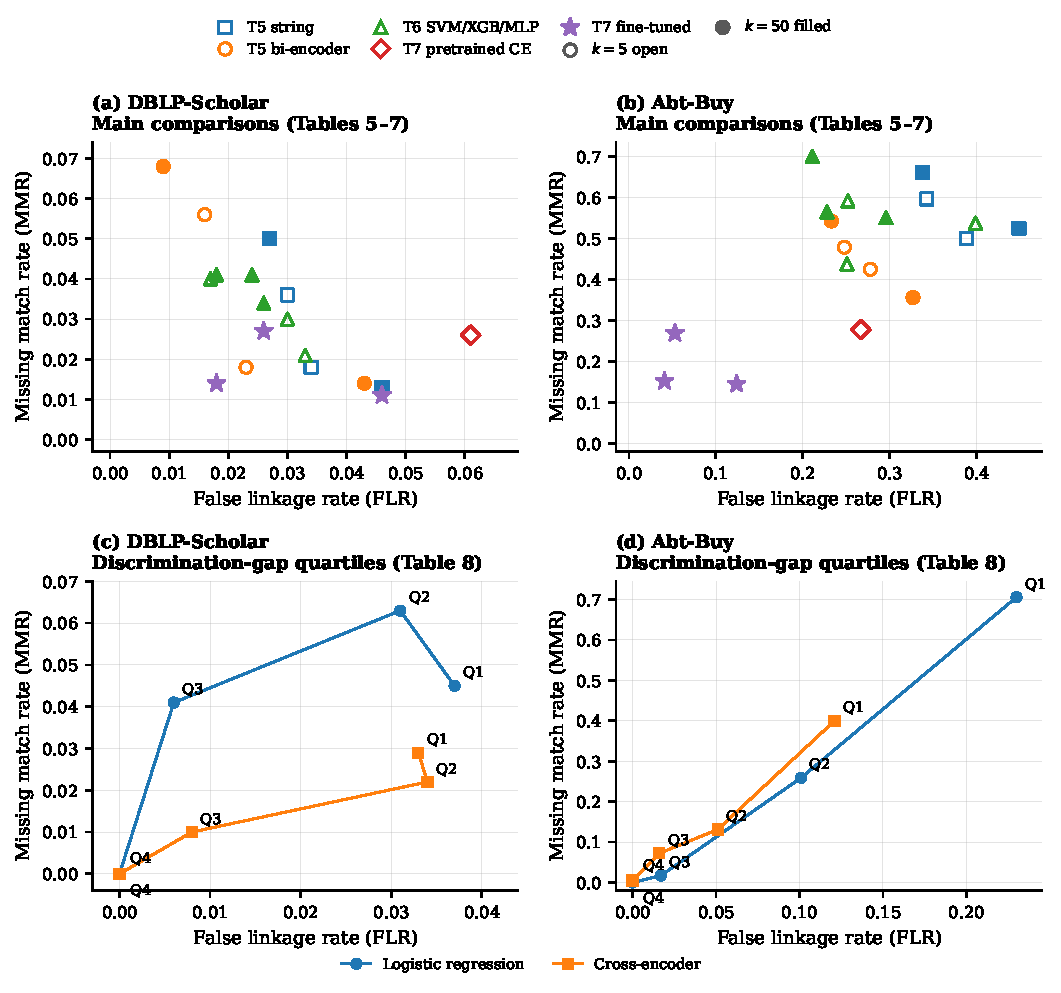
\includegraphics[width=0.98\textwidth]{flr_mmr_tradeoff.pdf}
\caption{\rev{Visual summary of the false linkage rate (FLR) and missing match rate
(MMR) tradeoff. Panels (a) and (b) summarise the main comparisons reported in
Tables~\ref{tab:comparison}--\ref{tab:fine-tuning} for DBLP-Scholar and Abt-Buy,
respectively. Panels (c) and (d) summarise the discrimination-gap quartile results
from Table~\ref{tab:discrimination-gap}. Points closer to the origin correspond to
lower error on both measures. The figure is intended as a descriptive complement to
the tables, which report the exact values and Monte Carlo standard errors.}}
\label{fig:flr-mmr-summary}
\end{figure}

\begin{figure}[ht]
\centering
\fbox{
\begin{minipage}{0.90\textwidth}
\centering
Texts
$\longrightarrow$
Embedding [transformer model]
$\longrightarrow$
Scoring [generative/discriminative model]

\vspace{0.8em}

$\longrightarrow$

Separate streams of harder cases and the rest

[e.g.\ by discrimination gap]

\vspace{0.8em}

$\longrightarrow$

\begin{tabular}{ll}
hard cases & $\longrightarrow$ Classification [cross-encoder] \\
rest       & $\longrightarrow$ Classification [generative/discriminative model]
\end{tabular}
\end{minipage}
}
\caption{Workflow of entity resolution combining different models. Type of model in
square brackets.}
\label{fig:combined-workflow}
\end{figure}

Figure \ref{fig:combined-workflow} shows the proposed workflow of entity
resolution with the additional details of how the traditional scoring models can be
combined with the transformer model. In particular, the workflow provides a way to
control the accuracy-cost tradeoff by using the traditional generative or
discriminative models to identify the hard cases for cross-encoder link
classification, while leaving the rest of the link classification to the traditional
model.

The potential computational saving arises because fine-tuning is performed once
for a given labelled sample, whereas the subsequent cost of cross-encoder
classification increases with the number of text pairs sent to it. Once the
bi-encoder embeddings have been obtained, scoring by the traditional models is
comparatively inexpensive. Routing only a subset of cases to the cross-encoder
therefore reduces the number of pairwise cross-encoder evaluations. \rev{As a
hardware-independent cost measure, Table~\ref{tab:combined-procedure} reports the
realised number of cross-encoder pair evaluations for the two training-derived routing
rules relative to sending all $k=50$ candidate pairs to the cross-encoder.} The realised
runtime saving will depend on the routing rule, block size, hardware and
implementation, and is not benchmarked systematically in the present paper.

Although the benefits of creating separate case streams for link classification and the
feasibility of using the traditional models for this task are clear by now, how to determine
exactly which cases should be sent to the cross-encoder model must depend on the cost
constraint and the acceptable accuracy in each application. It is also possible to consider
more refined schemes than, say, choosing a single threshold of the discrimination gap.

For instance, by MEC using a generative model, one can estimate both the FLR and MMR
for the classified link set, and use them to filter out the cases for the cross-encoder model.
Or, to further reduce the cost, one may consider sending fewer candidates for each case
passed on to the cross-encoder model, provided the left-out candidates have much lower
match probabilities than the selected ones according to the scoring model, in which
respect one may consider more refined discrimination measures than the gap
\eqref{eq:discrimination-gap} between the top two candidate match probabilities.

However, we notice that there is another issue related to the exact scheme of creating
separate case streams, which concerns the assessment of linkage errors by transformer
models, as we shall discuss in the next section. 
\rev{To demonstrate the combined
procedure directly, Section~\ref{sec:workable-error-assessment} also reports pooled
FLR and MMR under two routing rules whose discrimination-gap cutoffs are determined
from the training records and then applied unchanged to the test records.}


\subsection{Linkage error assessment of transformer models}
\label{sec:error-assessment}

Assessing the link classification errors of the cross-encoder model faces two major issues.
As we have explained in Section 1.2, the test errors only refer to the model fine-tuned on
the training set, which causes the first issue if one would like to fine-tune the model on the
whole labelled match sample using the hyperparameters settled on the training set, which
is a very common practice in Machine Learning \citep[e.g.][]{hastie2009elements}. The
second issue is related to the creation of separate case streams for link classification in the
proposed workflow, which means, for example, that the cross-encoder model would only be
applied to the selected harder cases instead of all the out-of-sample cases.

Below we investigate the first issue, before proposing a workable approach to linkage error
assessment, even though it does not yield unbiased estimation of the FLR and MMR.


\subsubsection{Sensitivity of training-test split}
\label{sec:split-sensitivity}

We have divided the sampled file-$A$ records into training and test sets 50--50 so far
in this paper. To study sensitivity to this choice, let $A_{s,f}$ denote an SRSWOR sample
containing a fraction $f=0.5,0.6,\ldots,0.9$ of the sampled file-$A$ records $A_s$, and let

\[
s_{M,f}
=
\{(i,j)\in s_M:i\in A_{s,f}\}
\]

denote the labelled match sample induced by those selected records. The cross-encoder is
trained using the records in $A_{s,f}$ and evaluated on the complementary file-$A$ records
$A_s\setminus A_{s,f}$, together with their associated gold-standard matches.

For each value of $f$, we repeat the random split ten times. The cross-encoder is
fine-tuned separately on each training sample using the same model and hyperparameters
as in Section \ref{sec:fine-tuning-models}. Within each training sample, 20\% of the
constructed training pairs are used as validation data to determine the link-classification
threshold by maximising the F1 score. The FLR and MMR are then evaluated on the
corresponding held-out file-$A$ records.

Table \ref{tab:training-fraction} reports the mean error rates over the ten replications,
together with their Monte Carlo standard errors. We also report the relative Monte Carlo
standard error, defined as the Monte Carlo standard error divided by the absolute mean
error rate, as an indication of the precision of the Monte Carlo mean.

\begin{table}[ht]
\centering
\caption{FLR and MMR of the cross-encoder model by training-set fraction $f$, based
on 10 replications. SE denotes the Monte Carlo standard error and RMCSE the relative
Monte Carlo standard error.}
\begin{tabular}{lrrrrrrr}
\toprule
& & \multicolumn{3}{c}{FLR} & \multicolumn{3}{c}{MMR} \\
\cmidrule(lr){3-5}\cmidrule(lr){6-8}
Dataset & $f$ & Mean & SE & RMCSE & Mean & SE & RMCSE \\
\midrule
DBLP-Scholar
& 0.5 & 0.017 & 0.001 & 0.058 & 0.015 & 0.001 & 0.077 \\
& 0.6 & 0.019 & 0.001 & 0.078 & 0.016 & 0.001 & 0.077 \\
& 0.7 & 0.014 & 0.002 & 0.136 & 0.015 & 0.002 & 0.110 \\
& 0.8 & 0.016 & 0.003 & 0.171 & 0.016 & 0.002 & 0.102 \\
& 0.9 & 0.015 & 0.003 & 0.188 & 0.019 & 0.002 & 0.115 \\
\addlinespace
Abt-Buy
& 0.5 & 0.039 & 0.003 & 0.064 & 0.160 & 0.005 & 0.033 \\
& 0.6 & 0.034 & 0.003 & 0.076 & 0.168 & 0.009 & 0.051 \\
& 0.7 & 0.029 & 0.004 & 0.133 & 0.164 & 0.004 & 0.026 \\
& 0.8 & 0.033 & 0.002 & 0.066 & 0.174 & 0.007 & 0.041 \\
& 0.9 & 0.029 & 0.004 & 0.148 & 0.158 & 0.013 & 0.080 \\
\bottomrule
\end{tabular}
\label{tab:training-fraction}
\end{table}

Table \ref{tab:training-fraction} gives the results from ten Monte Carlo
replications of the record-level training-test split for each given $f$. Although the FLR and MMR are not constant with respect
to the training-set size, there is no systematic improvement in either error rate as $f$
increases. For DBLP-Scholar, the mean FLR remains between approximately 0.014 and
0.019 over the five training fractions, while the MMR remains between approximately
0.015 and 0.019. For Abt-Buy, the FLR varies between approximately 0.029 and 0.039,
whereas the MMR varies between approximately 0.158 and 0.174.

The error rates can therefore be considered relatively stable over the range of training
fractions considered here, especially given the variability between random splits. At the
same time, increasing $f$ reduces the size of the holdout test set. For DBLP-Scholar,
the relative Monte Carlo standard error of the FLR becomes noticeably larger at the
higher training fractions. The corresponding RMCSE of the MMR is also somewhat
larger for several of the higher values of $f$, although the pattern is not monotonic.
For Abt-Buy, the relative Monte Carlo standard errors remain comparatively small for
most values of $f$, but increase for both error measures at $f=0.9$. Thus, allocating
more of the labelled sample to fine-tuning does not necessarily yield visibly lower test
error in these experiments, while it leaves fewer records for assessing that error.

However, the stability of the observed error rates does not solve the more fundamental
problem mentioned above. For any $f<1$, the test error in Table \ref{tab:training-fraction}
refers to the cross-encoder fine-tuned using the records in $A_{s,f}$, rather
than to a model subsequently fine-tuned using the complete sampled file-$A$
set $A_s$. Whether
the former can provide a useful estimate of the error of the latter is a separate question,
which we investigate next.


\subsubsection{Bias of subsample test error estimation}
\label{sec:subsample-bias}

We can explore the bias of subsample test error estimation for the larger-sample trained
cross-encoder model by the following setup. Let $A_{s,f}$ and the induced match sample
$s_{M,f}$ be given as above, with $A_s\setminus A_{s,f}$ providing the outer holdout
records. Now, treating $A_{s,f}$ as if it were the whole labelled file-$A$ sample, we create
an inner training sample $A^*_{s,f}\subset A_{s,f}$ and the corresponding inner test records.
Let $s^*_{M,f}$ denote the labelled match sample induced by $A^*_{s,f}$.

The sampling is therefore carried out at the level of file-$A$ records, with their associated
candidate blocks kept together. Let $\mathrm{FLR}$ denote the error of the model trained
using $A_{s,f}$ and evaluated on the outer holdout $A_s\setminus A_{s,f}$, which simulates
the target FLR of interest. Let $\mathrm{FLR}^*$ denote the error of the model trained using
$A^*_{s,f}$ and evaluated on the corresponding inner test records, which simulates
subsample test error estimation in practice. The replicate-level difference

\begin{equation}
\widehat{\mathrm{Bias}}_{\mathrm{FLR}}
=
\mathrm{FLR}^*-\mathrm{FLR}
\end{equation}

can then be used to assess the bias of the subsample test-set estimator. The same
construction is applied to the MMR,

\begin{equation}
\widehat{\mathrm{Bias}}_{\mathrm{MMR}}
=
\mathrm{MMR}^*-\mathrm{MMR}.
\end{equation}

We consider two choices of the inner training records $A^*_{s,f}$ given each
$A_{s,f}$. In addition to splitting $A_{s,f}$ by SRSWOR, we consider bootstrap
resampling, where a sample of size $|A_{s,f}|$ is drawn with replacement from the
file-$A$ records in $A_{s,f}$ and the source records not selected in the bootstrap sample
form the out-of-bag test set. Since a bootstrap sample of size $|A_{s,f}|$ contains on
average $1-e^{-1}\approx0.632$ distinct source records, we use a 65--35 training-test
split when constructing $A^*_{s,f}$ by SRSWOR for comparison.

\begin{table}[ht]
\centering
\caption{Bias of FLR and MMR estimation by sampling fraction $f$, using SRSWOR
or bootstrap subsampling. Results are based on 10 replications. Monte Carlo standard
errors (SE) of the estimated bias are given in parentheses.}
\label{tab:subsample-bias}
\begin{tabular}{llrrr}
\toprule
Dataset & $f$ & Target & SRSWOR bias (SE) & Bootstrap bias (SE) \\
\midrule
\multicolumn{5}{l}{\textit{Panel A: FLR}} \\[2pt]

DBLP-Scholar
& 0.5 & 0.017 & 0.003 (0.003) & 0.004 (0.002) \\
& 0.6 & 0.019 & 0.005 (0.003) & 0.003 (0.002) \\
& 0.7 & 0.014 & 0.005 (0.003) & 0.010 (0.003) \\
& 0.8 & 0.016 & 0.003 (0.004) & 0.008 (0.004) \\
& 0.9 & 0.015 & 0.004 (0.003) & 0.007 (0.003) \\

\addlinespace
Abt-Buy
& 0.5 & 0.039 &  0.001 (0.004) & 0.001 (0.006) \\
& 0.6 & 0.034 & -0.001 (0.006) & 0.004 (0.006) \\
& 0.7 & 0.029 &  0.007 (0.007) & 0.008 (0.006) \\
& 0.8 & 0.033 &  0.001 (0.005) & 0.001 (0.004) \\
& 0.9 & 0.029 &  0.004 (0.005) & 0.006 (0.006) \\

\midrule
\multicolumn{5}{l}{\textit{Panel B: MMR}} \\[2pt]

DBLP-Scholar
& 0.5 & 0.015 & -0.002 (0.001) &  0.005 (0.002) \\
& 0.6 & 0.016 & -0.001 (0.002) &  0.000 (0.002) \\
& 0.7 & 0.015 & -0.001 (0.003) &  0.003 (0.003) \\
& 0.8 & 0.016 &  0.001 (0.003) &  0.002 (0.003) \\
& 0.9 & 0.019 & -0.003 (0.003) & -0.003 (0.002) \\

\addlinespace
Abt-Buy
& 0.5 & 0.160 &  0.015 (0.012) &  0.010 (0.009) \\
& 0.6 & 0.168 &  0.015 (0.014) & -0.004 (0.013) \\
& 0.7 & 0.164 & -0.002 (0.008) &  0.007 (0.009) \\
& 0.8 & 0.174 & -0.007 (0.014) & -0.008 (0.008) \\
& 0.9 & 0.158 &  0.008 (0.018) &  0.007 (0.016) \\

\bottomrule
\end{tabular}
\end{table}

Table \ref{tab:subsample-bias} shows, for each outer training fraction
$f$, the target out-of-sample error and the estimated bias of the corresponding subsample
error under SRSWOR and bootstrap sampling. The results are averaged over ten Monte
Carlo replications, with the Monte Carlo SE of the bias estimator given in parentheses.

There are no large or systematic differences between the SRSWOR and bootstrap results.

\rev{For DBLP-Scholar, the estimated FLR biases are positive for all values of $f$ under both
sampling schemes, but the common sign should not be interpreted as evidence of a systematic
upward bias at this replication count. The estimates range from approximately 0.003 to 0.005
under SRSWOR and from approximately 0.003 to 0.010 under bootstrap sampling, and most
are within about one to two Monte Carlo standard errors of zero. Some of the bootstrap
estimates are larger relative to their Monte Carlo standard errors, but the ten-replication
experiment does not establish a common bias direction. The biases are nevertheless not
negligible relative to the very low target FLR for DBLP-Scholar.}

The corresponding MMR biases for DBLP-Scholar are generally smaller and do not have
a common direction. Under SRSWOR they range from approximately $-0.003$ to 0.001,
while under bootstrap sampling they range from approximately $-0.003$ to 0.005.
Several of the estimates are of similar magnitude to their Monte Carlo standard errors.

The picture is also mixed for Abt-Buy. The FLR biases are generally small and mostly
positive, with the exception of the SRSWOR result at $f=0.6$. The MMR bias changes
sign as $f$ varies under both sampling schemes, and its Monte Carlo standard error is
often large relative to the estimated bias. There is therefore no evidence here of a
common direction of bias that could simply be corrected by adding or subtracting a
fixed amount.

Overall, the results suggest that subsample test errors can provide a rough indication of
the error of a model trained on a larger labelled sample, but they should not be regarded
as unbiased estimates of that error. Nor do the results identify either SRSWOR or
bootstrap sampling as uniformly preferable. The difference between the model trained on
the subsample and the model trained on the larger labelled sample remains part of the
error-assessment problem.

\subsubsection{A workable approach to error assessment}
\label{sec:workable-error-assessment}

In light of the investigation above, a workable approach to linkage error assessment can
be given as follows. Assume the same partition of training and test sets for all the models,
and let $A_{\mathrm{test}}$ denote the file-$A$ records in the test set. Let

\[
A_{\mathrm{test}}^H \cup A_{\mathrm{test}}^R
=
A_{\mathrm{test}},
\qquad
A_{\mathrm{test}}^H \cap A_{\mathrm{test}}^R
=
\varnothing,
\]

denote the separation of hard and rest cases for link classification, where
$A_{\mathrm{test}}^H$ contains those selected for the fine-tuned cross-encoder model and
$A_{\mathrm{test}}^R$ the rest for link classification by the chosen generative or
discriminative model. \rev{For error assessment, the rule producing this partition must
be fixed using the training or validation data before the test set is evaluated; selecting
or tuning the rule from the test-set discrimination gaps or errors would make the
hard/rest split in-sample.} Let

\[
\phi
=
\frac{|A_{\mathrm{test}}^H|}
{|A_{\mathrm{test}}|}
\]

be the test-set proportion selected for cross-encoder classification. This quantity directly
describes the proportion of records routed to the more costly model and is therefore useful
for describing the computational cost of the combined procedure.

To estimate the linkage errors of the combined procedure, however, the component error
rates must be combined according to their respective denominators in Equation (1).
For $g\in\{R,H\}$, let

\[
C_g
=
\sum_{i\in A_{\mathrm{test}}^g\cap A(s_M)}
\ell_i y_{ij_i}
\]

denote the number of correctly linked matchable records in stratum $g$, let

\[
D_g
=
\sum_{i\in A_{\mathrm{test}}^g}\ell_i
\]

denote the number of declared links, and let

\[
M_g
=
|A_{\mathrm{test}}^g\cap A(s_M)|
\]

denote the number of matchable file-$A$ records. The linkage errors of the complete combined procedure are most directly
calculated by pooling the corresponding counts across the two strata. Provided that
at least one link is declared, the FLR and MMR are

\begin{equation}
\label{eq:combined-errors}
\widehat{\mathrm{FLR}}
=
1-\frac{C_R+C_H}{D_R+D_H},
\qquad
\widehat{\mathrm{MMR}}
=
1-\frac{C_R+C_H}{M_R+M_H}.
\end{equation}

This is simply Equation (1) applied to the link decisions produced by the complete
combined procedure.

\rev{To instantiate this procedure, we consider two explicit routing rules. For each
random split, the 25th or 50th percentile of the discrimination gaps among the outer
training records is used as the routing cutoff. The cutoff is therefore fixed before the
test set is evaluated. Test records with a gap at or below the cutoff are sent to the
fine-tuned cross-encoder, while the remaining records are classified by logistic
regression using the fine-tuned bi-encoder similarities. Because the distribution of gaps
may differ between the training and test records, the realised test-set routing proportion
$\phi$ need not equal 0.25 or 0.50. Table~\ref{tab:combined-procedure} reports the
resulting pooled error rates from Equation~\eqref{eq:combined-errors}.}

\begin{table}[ht]
\centering
\caption{\rev{Combined-procedure error rates under training-derived discrimination-gap
routing rules. Entries for $\phi$, FLR and MMR give the mean (Monte Carlo standard
error) over seeds 42--44. Cross-encoder evaluations are the mean number of routed
record pairs per split for $k=50$, relative to evaluating all 50 candidates for every test
record; the percentage in parentheses is the corresponding reduction.}}
\scriptsize
\setlength{\tabcolsep}{4pt}
\begin{tabular}{llrrrr}
\toprule
Dataset & Training-gap rule & $\phi$ & FLR & MMR & Cross-encoder evaluations \\
\midrule
DBLP-Scholar & 25th percentile & \rev{0.246 (0.0033)} & \rev{0.017 (0.0018)} & \rev{0.033 (0.0025)} & \rev{16,117 / 65,400 (75.4\%)} \\
             & 50th percentile & \rev{0.485 (0.0123)} & \rev{0.017 (0.0034)} & \rev{0.024 (0.0035)} & \rev{31,700 / 65,400 (51.5\%)} \\
\addlinespace
Abt-Buy      & 25th percentile & \rev{0.333 (0.0115)} & \rev{0.050 (0.0035)} & \rev{0.148 (0.0048)} & \rev{9,000 / 27,050 (66.7\%)} \\
             & 50th percentile & \rev{0.590 (0.0149)} & \rev{0.042 (0.0021)} & \rev{0.145 (0.0138)} & \rev{15,950 / 27,050 (41.0\%)} \\
\bottomrule
\end{tabular}
\label{tab:combined-procedure}
\end{table}

\rev{The two rules exhibit the intended accuracy-cost tradeoff directly. For
DBLP-Scholar, the 50th-percentile training-gap rule routes 0.485 of the test records on
average and reduces cross-encoder pair evaluations by 51.5\%, with pooled FLR 0.017
and MMR 0.024. The corresponding Abt-Buy rule routes 0.590 of the test records and
reduces cross-encoder evaluations by 41.0\%, with pooled FLR 0.042 and MMR 0.145.
For reference, applying the fine-tuned cross-encoder to all test records in
Table~\ref{tab:fine-tuning} gives FLR/MMR 0.018/0.014 for DBLP-Scholar and
0.041/0.152 for Abt-Buy, whereas fine-tuned logistic regression gives 0.026/0.027 and
0.053/0.269, respectively. The 25th-percentile rule reduces cross-encoder evaluations
further, at the cost of a different balance between FLR and MMR. These results are
illustrative of the two training-derived routing rules rather than an optimisation over
possible cutoffs.}

For a stratum $g\in\{R,H\}$ with positive relevant denominators, the component
error rates can also be written as

\[
\widehat{\mathrm{FLR}}_g
=
1-\frac{C_g}{D_g},
\qquad
\widehat{\mathrm{MMR}}_g
=
1-\frac{C_g}{M_g}.
\]

When the component denominators are positive, Equation
\eqref{eq:combined-errors} is equivalently

\[
\widehat{\mathrm{FLR}}
=
\frac{D_R}{D_R+D_H}
\widehat{\mathrm{FLR}}_{\mathrm{rest}}
+
\frac{D_H}{D_R+D_H}
\widehat{\mathrm{FLR}}_{\mathrm{cross}},
\]

and

\[
\widehat{\mathrm{MMR}}
=
\frac{M_R}{M_R+M_H}
\widehat{\mathrm{MMR}}_{\mathrm{rest}}
+
\frac{M_H}{M_R+M_H}
\widehat{\mathrm{MMR}}_{\mathrm{cross}}.
\]

Writing the pooled counts first also covers the case in which one routed stratum
declares no links, so that its stratum-specific FLR is undefined even though the
FLR of the complete combined procedure remains well-defined.

In other words, treat $A_{\mathrm{test}}^R$ as the auditing sample for the traditional
model and $A_{\mathrm{test}}^H$ as that for the fine-tuned cross-encoder model. The
difference from evaluating either model alone is that the error assessment follows the same
routing rule that would be used in application. Hence the resulting FLR and MMR refer to
the combined linkage procedure actually being considered.

Notice that the routing proportion $\phi$ is not generally the appropriate weight for both
error rates. For the MMR it coincides with the weight in
Equation \eqref{eq:combined-errors} when all test records are matchable. For the FLR,
the relevant weights depend instead on the numbers of links declared by the two models.
This follows directly from the different denominators of FLR and MMR in Equation (1).

The estimates in Equation \eqref{eq:combined-errors} can be used to assess the linkage
errors of the procedure in which the models learned from the training set are subsequently
applied without change outside the labelled sample. This includes the fine-tuned
bi-encoder and cross-encoder models, the chosen generative or discriminative model, and
the rule used to separate the hard cases from the rest.

The matter is less straightforward if some or all of the models are subsequently retrained
using the complete labelled sample before out-of-sample deployment. In that case, the
test-set estimates refer to models trained on less data than the models eventually deployed.
If the full-sample retrained models have lower linkage errors, the test-set estimates may be
conservative. However, the results in Section \ref{sec:subsample-bias} show that the
direction and magnitude of this discrepancy need not be the same for FLR and MMR or
across applications. Bias exploration following the setup of that section can therefore be
used to gather the relevant evidence.

Thus, the approach does not remove the general difficulty of estimating the error of a
model that is retrained after evaluation. It provides a workable error assessment for the
combined entity-resolution procedure while preserving the separation between the
traditional model and the cross-encoder that is required for the accuracy-cost tradeoff.




% =========================================================
% SECTION 4
% Final remarks
% =========================================================

\section{Final remarks}
\label{sec:final-remarks}

The traditional workflow may yield high error rates for entity resolution based on more or
less free texts, because hand-crafted preprocessing rules and traditional scoring models
cannot handle natural language as effectively as structured linkage key values.

The transformer-only workflow, on the other hand, may not be scalable in many
applications, because the cross-encoder model needs to handle a potentially large number
of text pairs directly. Assessment of the associated linkage errors presents another
challenge in practice, particularly when the available labelled sample is used both for
fine-tuning and for error assessment.

The proposed workflow replaces hand-crafted text processing by automated bi-encoder
embedding and refines the steps of scoring and classification (Figure
\ref{fig:combined-workflow}). This allows one to deploy the cross-encoder model to only
a subset of selected cases, while capitalising on the cost-effective baseline performance
that is achievable by the traditional generative or discriminative models. The combined use of the models provides a practical mechanism for controlling
the tradeoff between linkage accuracy and computational cost.

The empirical results illustrate the different roles of the components in this workflow.
Bi-encoder embeddings can improve on traditional string comparisons, especially for
messier texts such as those in Abt-Buy. Fine-tuning can further improve the bi-encoder
representation, although the effect depends on both the dataset and the scoring model.
The fine-tuned cross-encoder yields a favourable balance between FLR and MMR on both
datasets, but at a higher computational cost. The discrimination-gap results show that cross-encoder evaluations can be
concentrated on the harder cases, while many of the easier cases can remain with the
traditional scoring-classification model. 
\rev{The explicit combined-procedure experiment
makes this tradeoff concrete: using the 50th percentile of the training-record gaps as the
routing cutoff reduces cross-encoder pair evaluations by 51.5\% for DBLP-Scholar and
41.0\% for Abt-Buy, with pooled FLR/MMR of 0.017/0.024 and 0.042/0.145,
respectively.}

\rev{The empirical findings are based on two benchmark datasets, and the extent to which the observed patterns generalise to other entity-matching settings remains to be assessed.}

The issues of linkage error assessment have also been studied. Test-set error estimates
refer directly to the models fitted on the corresponding training samples, and need not
equal the errors of models subsequently retrained on a larger labelled sample. The
subsample experiments show that the discrepancy is not of a common direction for both
FLR and MMR. A workable approach is therefore to assess the combined procedure under
the same routing rule that will be used for classification, using the appropriate
denominators of FLR and MMR for combining the component errors. If the component
models are subsequently retrained on the complete labelled sample, additional assumptions
or evidence are needed to relate these test-set estimates to the errors of the retrained
models.

Let us close by outlining three topics for future research on using transformer models for
entity resolution.

The first topic concerns embedding. As noted before, a weakness of the bi-encoder is
that it must encode each text $\tau_i$ without ``seeing'' the other similar texts, including
the likely matched item (Table \ref{tab:silverman-example}). \citet{morris2025contextual} propose a contextual document embedding (CDE) model,
which first uses a sample of texts from the same domain to create a domain-specific
contextual sequence, say $\xi$, and then encodes each concatenated item
$(\xi,\tau_i)$, instead of just $\tau_i$ on its own. The embedding
$\mathbf{x}(\xi,\tau_i)$ may improve on $\mathbf{x}(\tau_i)$ given an appropriate
$\xi$, while using a common $\xi$ for every item keeps the computation scalable.
Whether the particular CDE model, or other ideas of contextual embedding, can be
successfully implemented for entity resolution is clearly worth studying.

Secondly, scoring-classification in the unsupervised setting is a topic we did not consider
in this paper. In particular, fine-tuning of the cross-encoder model would remain
necessary if it is to be adapted to the texts of a specific application. One possibility is
to create a pseudo match sample $\widetilde{s}_M$, where a traditional model is used to
obtain automatically a link set for $A_s$ with a sufficiently low estimated FLR, and use
it as if it were a labelled match sample $s_M$. How reliable such pseudo-labels must be,
and how their errors propagate through fine-tuning and subsequent classification, would
need to be investigated. More generally, the application of cross-encoder models in the
unsupervised setting remains an open question.

Finally, the workflow configuration itself may be refined. In particular, one can study how
best to create separate case streams for link classification, including the possibilities
discussed in Section \ref{sec:combining-models}. The choice is intrinsically connected to
the accuracy-cost tradeoff. Computational cost can be evaluated relatively directly, but
the associated linkage error rates are more difficult to assess, both conceptually and
practically. We have proposed a workable approach in the supervised setting and a setup
for exploring the potential discrepancy between subsample and larger-sample error
assessment in Section \ref{sec:subsample-bias}. Corresponding methods for error
assessment in the unsupervised setting are still needed when entity resolution involves
the use of transformer models.

% =========================================================
% DATA AND CODE AVAILABILITY
% =========================================================

\section*{Data and code availability}
\rev{The DBLP-Scholar and Abt-Buy benchmark datasets are publicly available through the Magellan data repository cited in Appendix~\ref{app:datasets}. The supplementary reproduction package supplied with this revision contains the data files used in the analyses, scripts for blocking, embedding, fine-tuning, scoring, routing and error assessment, the random seeds, pinned core software versions, and a single entry point (\texttt{python reproduce.py}) for regenerating Tables~4--10. The main comparisons use seeds 42--44, while the training-fraction and nested error-assessment analyses use seeds 42--51. Revision-specific code and per-seed outputs for the updated Table~8 and the combined-procedure analysis are also included. GPU fine-tuning is not assumed to be bitwise deterministic across software and hardware stacks; the package therefore records the final environment and per-seed outputs used to assess numerical reproduction. A permanent archive identifier can be added to the accepted version.}

% =========================================================
% APPENDIX
% =========================================================

\appendix

% ============================================================
% Appendix A — Datasets
% ============================================================

\section{Datasets}
\label{sec:appendix-datasets}
\label{app:datasets}

Two benchmark datasets from the Magellan data repository
\citep{konda2016magellan} are used throughout the paper, one for
bibliographic citation matching and one for product matching.
Both have been widely used in the entity resolution literature
\citep[e.g.][]{mudgal2018deep, li2020deep, peeters2021dual}.
The Magellan data repository is available at
\url{https://pages.cs.wisc.edu/~anhai/data1/magellan_data/}.

\paragraph{DBLP-Scholar}
Let file $A$ contain $2{,}616$ publication records from the DBLP
computer science bibliography, and let file $B$ contain $64{,}263$
records from Google Scholar. Records in both files have four fields:
title, author, venue, and year.

The labelled match set contains $5{,}347$ record pairs involving
$2{,}408$ distinct records from $A$ and $5{,}218$ distinct records
from $B$. The match relation is not one-to-one:
$1{,}238$ matched records in $A$ have more than one valid partner in
$B$, and the largest number of valid partners for a single record is
20. All $5{,}347$ labelled pairs refer to records that are present in
the two files.

For supervised learning, one valid file-$B$ partner is retained as
the positive example for each matched file-$A$ record. Any other
known valid partners of the same file-$A$ record are excluded from
the non-match examples. The complete labelled match relation is
retained for evaluation, so that a predicted link is counted as
correct if the selected file-$B$ record is any of the known valid
partners of the corresponding file-$A$ record.

\paragraph{Abt-Buy}
Let file $A$ contain $1{,}081$ product records from Abt.com, and let
file $B$ contain $1{,}092$ records from Buy.com. The Abt file contains product name, description and price, while the Buy file
additionally contains manufacturer. The price field is not used in the calculations in this
paper.

The labelled match set contains $1{,}097$ record pairs. All
$1{,}081$ records in $A$ have at least one valid match, and all
$1{,}092$ records in $B$ occur in the labelled match set. Sixteen
records in $A$ have two valid partners in $B$, while all remaining
records have one. As for DBLP-Scholar, one valid partner is retained
per file-$A$ record for supervised training, while all known valid
partners are retained when determining whether a predicted link is
correct.



% =========================================================
% REFERENCES
% =========================================================

\clearpage

\bibliographystyle{apalike}
\bibliography{references}

\end{document}

